\section{Paper III: Neural network analysis of sleep stages enables efficient diagnosis of narcolepsy}\label{sec:paperiii}
\sectionmark{Stephansen \& Olesen, \textit{et al.}, 2018}

\begin{tcolorbox}[colframe=white]
\paragraph{Abstract:} Analysis of sleep for the diagnosis of sleep disorders such as \ac{NT1} currently requires visual inspection of polysomnography records by trained scoring technicians. 
Here, we used neural networks in approximately \num{3000} normal and abnormal sleep recordings to automate sleep stage scoring, producing a hypnodensity graph---a probability distribution conveying more information than classical hypnograms. 
Accuracy of sleep stage scoring was validated in 70 subjects assessed by six scorers. 
The best model performed better than any individual scorer (87\% versus consensus). 
It also reliably scores sleep down to \SI{5}{\second} instead of \SI{30}{\second} scoring epochs.
% A \ac{NT1} marker based on unusual sleep stage overlaps achieved a specificity of 96\% and a sensitivity of 91\%, validated in independent datasets. 
% Addition of \hla typing increased specificity to 99\%. 
% Our method can reduce time spent in sleep clinics and automates \ac{NT1} diagnosis. 
% It also opens the possibility of diagnosing \ac{NT1} using home sleep studies.
\end{tcolorbox}

\subsection{Materials \& Methods}

\subsubsection{Datasets}
The success of machine learning depends on the size and quality of the data on which the model is trained and evaluated~\cite{Banko2001, Shotton2011}.
We used a large dataset comprised of several thousand sleep studies to train, validate, and test/replicate our models.
To ensure heterogeneity, data came from 4 different cohorts: \ac{SSC}~\cite{Andlauer2013, Moore2014}, \ac{WSC}~\cite{Moore2014, Young2009}, \ac{IS-RC}~\cite{Kuna2013}, and \ac{KHC}~\cite{Hong2006}
Institutional Review Boards approved the study and informed consent was obtained from all participants.
Technicians trained in sleep scoring manually labeled all sleep studies.
\Cref{fig:sleep-stages:paper-iii:figure-05}a and b summarize the overall design of the study for sleep stage scoring.
\Cref{tab:sleep-stages:paper-iii:table-s01} provides a summary of the size of each cohort and how it was used.
% In the narcolepsy biomarker aspect of the study, \acp{PSG} from \ac{NT1} and other patients were split across most datasets to ensure heterogeneity in both the training and testing dataset.
For this analysis, a few recordings with poor quality sleep studies, i.e. missing critical channels, with additional sensors or with a too short sleep duration ($\leq \SI{2}{\hour}$) were excluded.
% A “never seen” subset cohort that included French and Chinese subjects (FHC and CNC) was also tested.
Below is a brief description of each dataset.

\paragraph{Population-based Wisconsin Sleep Cohort}
This cohort is a longitudinal study of state agency employees aged 37--82 years from Wisconsin, USA, and approximates a population-based sample (see~\cref{tab:sleep-stages:paper-iii:table-s01} for age at study).
The subjects in this study are generally more overweight~\cite{Young2009}.
The study is ongoing, and dates back to 1988.
2167 \acp{PSG} in 1086 subjects were used for training while 286 randomly selected \acp{PSG} were used for validation testing of the sleep stage-scoring algorithm.% and narcolepsy biomarker training.
Approximately 25\% of the population have an \ac{AHI} above \SI{15}{\hour} and 40\% have a \ac{PLMI} above \SI{15}{\hour}.
A detailed description of the sample can be found in~\cite{Young2009} and~\cite{Moore2014}.
%The sample does not contain any \ac{NT1} patients, and the three subjects with possible \ac{NT1} were removed~\cite{Goldbart2014}.

\begin{table}[tb]
\centering
% \begin{adjustwidth*}{}{-\marginparwidth-\marginparsep}
\begin{threeparttable}  
\small
\caption[\acs{STAGES} cohorts]{Description of the various cohorts included in this study.}
\label{tab:sleep-stages:paper-iii:table-s01}
\begin{tabular}{@{}lcccccc@{}}
    \toprule
    \textbf{Cohort}         & \textbf{Age, years}       & \textbf{BMI, \si{\kilogram\per\meter\squared}}        & \textbf{Sex, \%}       & \textbf{Train}      & \textbf{Test}      \\ \midrule
    \ac{WSC}            & 59.7 $ \pm $ 8.4  & 31.6 $ \pm $ 7.1  & 53.1      & 1086 (2167)        & 286 \\
    \ac{SSC}            & 45.4 $ \pm $ 13.8 & 23.9 $ \pm $ 6.5  & 59.4      & 617                & 277 \\
    \ac{KHC}            & 29.1 $ \pm $ 13.2 & 24.1 $ \pm $ 4.3  & 58.6      & None               & 160 \\
    \ac{IS-RC}          & 51.1 $ \pm $ 4.2  & 32.9 $ \pm $ 9.2  & 0         & None               & 70 \\ \midrule
    Total subjects &                    &                   &           & 1703              & 793 \\
    Total \acsp{PSG} &                    &                   &           & 2784              & 793 \\ \bottomrule
\end{tabular}
\begin{tablenotes}
\small \item Variables are aggregated across \acp{PSG}. %
\describe{WSC}; %
\describe{SSC}; %
\describe{KHC}; %
\describe{IS-RC}.
\end{tablenotes}
\end{threeparttable}
% \end{adjustwidth*}
\end{table}

\paragraph{Patient-based Stanford Sleep Cohort}
\acp{PSG} from this cohort were recorded at the Stanford Sleep Clinic dating back to 1999, and represent sleep disorder patients aged 18-91 visiting the clinic (see~\cref{tab:sleep-stages:paper-iii:table-s01} for age at study).
The cohort contains thousands of \ac{PSG} recordings, but for this study we used 894 diagnostic (no positive airway pressure (PAP)) recordings in independent patients that have been used in prior studies~\cite{Kuna2013}.
This subset contains patients with a range of different diagnoses including: sleep disordered breathing (607), insomnia (141), \ac{REM} sleep behavior disorder (4), restless legs syndrome (23), \ac{NT1} (25), delayed sleep phase syndrome (14), and other conditions (39).
Description of the subsample can be found in~\cite{Andlauer2013} and~\cite{Moore2014}.
Approximately 30\% of subjects have an \ac{AHI} above \SI{15}{\hour}, or a \ac{PLMI} above \SI{15}{\hour}.
617 randomly selected subjects were used for training the neural networks while 277 randomly selected \acp{PSG} were kept for validation testing of the sleep stage scoring algorithm.
%These 277 subjects were also used for training the narcolepsy biomarker algorithm.
%The sample contains \acp{PSG} of 25 independent untreated subjects with \ac{NT1} (12 with low CSF hypocretin-1, the others with clear cataplexy).
26 subjects were removed from the study---4 due to poor data quality, and the rest due to continued medication usage.

\paragraph{Patient-based Korean Hypersomnia Cohort}
The Korean Hypersomnia Cohort is a high pretest probability sample for narcolepsy.
It includes 160 patients with a primary complaint of excessive daytime sleepiness (see~\cref{tab:sleep-stages:paper-iii:table-s01} for age at study).
These \acp{PSG} were used for testing the sleep scoring algorithm.% and for training the narcolepsy biomarker algorithm.
No data was used for training the sleep-scoring algorithm.
Detailed description of the sample can be found in~\cite{Hong2006} and~\cite{Andlauer2013}.
%The sample contains \acp{PSG} of 66 independent untreated subjects with \ac{NT1} and clear cataplexy.
%Two subjects were removed from the narcolepsy biomarker study because of poor data quality.

\paragraph{Patient-based Inter-scorer Reliability Cohort}
As~\citeauthor{Rosenberg2013}~\cite{Rosenberg2013} have shown, variation between individual scorers can sometimes be large, leading to an imprecise gold standard.
To quantify this, and to establish a more accurate gold standard, 10 scorers from five different institutions, University of Pennsylvania, St. Luke’s Hospital, University of Wisconsin at Madison, Harvard University, and Stanford University, analyzed the same 70 full night \acp{PSG}.
This allowed for a much more precise gold standard, and the inter-scorer reliability could be quantified for a dataset, which could also be examined by automatic scoring algorithms.
For this study, scoring data from University of Pennsylvania, St. Luke’s and Stanford were used.
All subjects are female (see~\cref{tab:sleep-stages:paper-iii:table-s01} for details).
Detailed description of the sample can be found in~\cite{Kuna2013} and~\cite{Malhotra2014}.
% The sample does not contain any \ac{NT1} patients.

\paragraph{American Academy of Sleep Medicine Sleep Study}
The \ac{AASM} ISR dataset is composed of a single control sleep study of 150 epochs of each \SI{30}{\second} in length that was scored by \plusminus{5234}{14} experienced sleep technologists for quality control purposes.
Design of this dataset is described in~\cite{Rosenberg2013}.

\begin{figure}[t]
\begin{adjustwidth*}{}{-\marginparwidth-\marginparsep}
    \myfloatalign   
    \subfloat[]
    {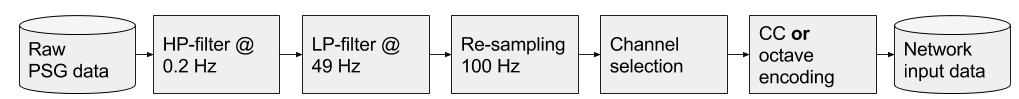
\includegraphics[width=\linewidth]{figures/paper-iii/Figure_5a.png}}  \\
    \subfloat[]
    {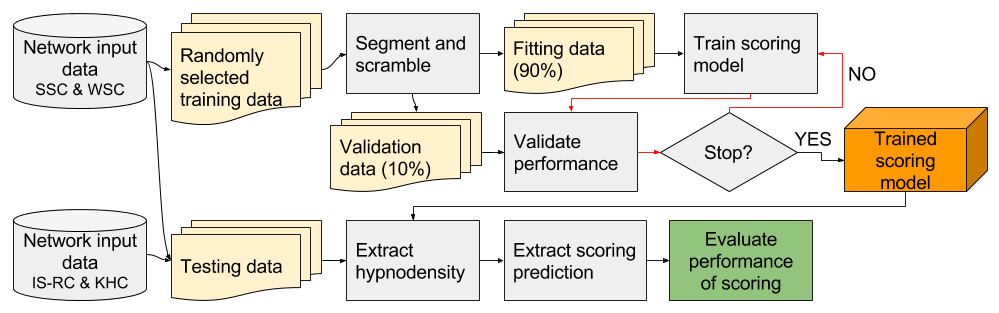
\includegraphics[width=\linewidth]{figures/paper-iii/Figure_5b.png}}
    \caption[\acs{STAGES} model for sleep staging]{Overview of \ac{STAGES} model for sleep stage classification. (a) Pre-processing steps taken to achieve the format of data as it is used in the neural networks. One of the 5 channels is first high-pass filtered with a cut-off at \SI{0.2}{\hertz}, then low-pass filtered with a cut-off at \SI{49}{\hertz} followed by a re-sampling to \SI{100}{\hertz} to ensure data homogeneity. In the case of \ac{EEG} signals, a channel selection is employed to choose the channel with the least noise. The data are then encoded using either the \ac{CC} or the octave encoding. (b) Producing and testing the automatic scoring algorithm. A part of the \ac{SSC}~\cite{Andlauer2013,Moore2014} and \ac{WSC}~\cite{Moore2014, Young2009} is randomly selected, as described in~\cref{tab:sleep-stages:paper-iii:table-s01}. These data are then segmented in 5 min segments and scrambled with segments from other subjects to increase batch similarity during training. A neural network is then trained until convergence (evaluated using a separate validation sample). Once trained, the networks are tested on a separate part of the \ac{SSC} and \ac{WSC} along with data from the \ac{IS-RC}~\cite{Kuna2013} and \ac{KHC}~\cite{Andlauer2013, Hong2006}.}
    \label{fig:sleep-stages:paper-iii:figure-05}
\end{adjustwidth*}
\end{figure}

\subsubsection{Data labels, scoring and fuzzy logic}
Sleep stages were scored by \ac{PSG}-trained technicians using established scoring rules, as described in the \ac{AASM} Scoring Manual~\cite{Berry2017}.
In doing so, technicians assign each epoch with a discrete value.
With a probabilistic model, like the one proposed in this study, a relationship to one of the fuzzy sets is inferred based on thousands of training examples labeled by many different scoring-technicians. 

The hypnodensity graph refers to the probability distribution over each possible stage for each epoch, as seen in~\cref{fig:sleep-stages:paper-iii:figure-02a,fig:sleep-stages:paper-iii:figure-02b}.
This allows more information to be conveyed, since every epoch of sleep within the same stage is not identical. 
For comparison with the gold standard, however, a discrete value must be assigned from the model output as:
\begin{equation}
    \hat{y} = \argmax_{\mathbf{y}_{i}} \sum_{i}^{N} \mathbf{P}_i \parentheses{ \mathbf{y}_i \! \mid \! \mathbf{x}_i },
\end{equation}
where $\mathbf{P}_i \parentheses{ \mathbf{y}_i \! \mid \! \mathbf{x}_i }$ is a vector with the estimated probabilities for each sleep stage in the \textit{i}th segment, $N$ is the number of segments an epoch is divided into, and $\hat{y}$ is the estimated label. 

Sleep scoring technicians score sleep in \SI{30}{\second} epochs, based on what stage they assess is represented in the majority of the epoch---a relic of when recordings were done on paper. 
This means that when multiple sleep stages are represented, more than half of the epoch may not match the assigned label. 
This is evident in the fact that the label accuracy decreases near transition epochs~\cite{Rosenberg2013}.
One solution to this problem is to remove transitional regions to purify each class. 
However, this has the disadvantage of under-sampling transitional stages, such as \ac{N1}, and removes the context of quickly changing stages, as is found in a spontaneous arousal. 
It has been demonstrated that the negative effects of imperfect “noisy” labels may be mitigated if a large enough training dataset is incorporated and the model is robust to overfitting~\cite{Caruana2000}.
This also assumes that the noise is randomly distributed with an accurate mean---a bias cannot be canceled out, regardless of the amount of training data. 
For these reasons, all data including those containing sleep transitions were included. 
Biases were evaluated by incorporating data from several different scoring experts cohorts and types of subjects.

To ensure quick convergence, while also allowing for long-term dependencies in memory-based models, the data were broken up in \SI{5}{\minute} blocks and shuffled to minimize the shift in covariates during training caused by differences between subjects. 
To quantify the importance of segment sizes, both \SI{5}{\second} and \SI{15}{\second} windows were also tested.

% \begin{landscape}
% \begin{table}[tb]
% \begin{threeparttable}  
% \small
% \centering
% \caption[\acs{STAGES} cohorts]{Description of the various cohorts included in this study and how they were used.}
% \label{tab:sleep-stages:paper-iii:table-s01}
% \begin{tabular}{@{}lccccccccccc@{}}
%     \toprule
%     & & & & \multicolumn{2}{c}{Sleep scoring} & \multicolumn{3}{c}{Narcolepsy biomarker} & & & \\ \cline{5-6} \cline{7-9}
%     Cohort         & Age, $ \mu \pm \sigma $        & BMI, $ \mu \pm \sigma $        & Sex, \% male       & Train      & Test      & Train  & Test              & Replication            & \% narco & \% hypersomnia \\ \midrule
%     \ac{WSC}            & 59.7 $ \pm $ 8.4  & 31.6 $ \pm $ 7.1  & 53.1      & 1086 (2167~\acp{PSG}) & 286  & 170                  & 116          & None        & 0        & 0 \\
%     \ac{SSC}            & 45.4 $ \pm $ 13.8 & 23.9 $ \pm $ 6.5  & 59.4      & 617                & 277  & 139                  & 112          & None        & 11.6     & 1.8 \\
%     \ac{KHC}            & 29.1 $ \pm $ 13.2 & 24.1 $ \pm $ 4.3  & 58.6      & None               & 160  & 87                   & 71           & None        & 45.8     & 54.2 \\
%     AHC            & 34.5 $ \pm $ 13.8 & 25.9 $ \pm $ 4.9  & 54        & None               & None & 42 (76~\acp{PSG})         & 44 (84~\acp{PSG}) & None        & 52.3     & 47.7 \\
%     \ac{IS-RC}          & 51.1 $ \pm $ 4.2  & 32.9 $ \pm $ 9.2  & 0         & None               & 70   & None                 & None         & None        & 0        & 0 \\
%     JCTS           & 53.2 $ \pm $ 9.8  & 31.0 $ \pm $ 4.4  & 57.1      & None               & None & 7                    & None         & None        & 100      & 0 \\
%     IHC            & 33.7 $ \pm $ 17.6 & -           & 56.7      & None               & None & 87                   & 61           & None        & 47.3     & 50 \\
%     DHC            & 33.4 $ \pm $ 14.8 & 24.8 $ \pm $ 4.9  & 50        & None               & None & 79                   & None         & None        & 26.6     & 48.1 \\
%     FHC            & 28.8 $ \pm $ 15.2 & 24.4 $ \pm $ 8.1  & 59        & None               & None & None                 & None         & 122         & 51.6     & 18 \\
%     CNC            & 28.5 $ \pm $ 16.9 & 23.2 $ \pm $ 11.5 & 51.3      & None               & None & None                 & None         & 199         & 34.2     & 0 \\ \midrule
%     Total subjects &             &             &           & 1,703              & 793  & 611                  & 404          & 321         &          & \\
%     Total \acp{PSG}     &             &             &           & 2,784              & 793  & 645                  & 444          & 321         &          & \\ \bottomrule
% \end{tabular}
% \begin{tablenotes}
% \footnotesize
% \item \ac{WSC}, \ac{SSC} \quad Training and testing of sleep scoring models and narcolepsy biomarker.
% \item \ac{KHC} \quad Sleep scoring testing, and training and testing of narcolepsy biomarker.
% \item AHC \quad Training and testing of narcolepsy biomarker. 86 subjects had the first \ac{PSG} recorded, and 75 had an additional second \ac{PSG}.\newline A subject was used for either training or testing.
% \item \ac{IS-RC} \quad Scored by 6 different scorers. Final assessment and validation of predictive performance for sleep scoring.
% \item JCTS, DHC \quad Training of narcolepsy biomarker.
% \item IHC \quad Training and testing of narcolepsy biomarker.
% \item FHC, CNC \quad Replication of narcolepsy biomarker. 
% \end{tablenotes}
% \end{threeparttable}
% \end{table}
% \end{landscape}

\subsubsection{Data selection and pre-processing}
A full night \ac{PSG} \textsc{psg} involves recording many different channels, some of which are not necessary for sleep scoring~\cite{Silber2007}\graffito{The \acs{AASM} recommends \acs{EEG}, \acs{EOG}, and chin \acs{EMG} for sleep stage scoring, see~\cref{sec:polysomnography}.}. 
In this study, \ac{EEG} (C3 or C4, and O1 or O2), chin \ac{EMG}, and the left and right \ac{EOG} channels were used, with reference to the contralateral mastoid. 
Poor electrode connections are common when performing a \ac{PSG} analysis. 
This can lead to a noisy recording, rendering it useless. 
To determine whether right or left \ac{EEG} channels were used, the noise of each was quantified by dividing the \ac{EEG} data in \SI{5}{\minute} segments, and extracting the Hjorth parameters~\cite{Hjorth1970}. 
These were then log-transformed, averaged, and compared with a previously established multivariate distribution, based on the \ac{WSC}~\cite{Young2009,Moore2014} and \ac{SSC}~\cite{Andlauer2013,Moore2014} training data. 
The channel with lowest Mahalanobis distance to this distribution was selected. 
The log-transformation has the advantage of making flat signals/disconnects as uncommon as very noisy signals, in turn making them less likely to be selected. 
To minimize heterogeneity across recordings, and at the same time reducing the size of the data, all channels were down-sampled to \SI{100}{\hertz}. 
Additionally, all channels were filtered with a \nth{5} order two-directional \ac{IIR} high-pass filter with cutoff frequency of \SI{0.2}{\hertz} and a \nth{5} order two-directional \ac{IIR} low-pass filter with cutoff frequency of \SI{49}{\hertz}. 
The \ac{EMG} signal contains frequencies well above \SI{49}{\hertz}, but since much data had been down-sampled to \SI{100}{\hertz} in the \ac{WSC}, this cutoff was selected for all cohorts. 
All steps of the pre-processing are illustrated in~\cref{fig:sleep-stages:paper-iii:figure-05}a.

\subsubsection{Convolutional and recurrent neural networks}
\acp{CNN} are a class of deep learning models initially developed to solve problems in the field of computer vision~\cite{LeCun2015}.
A \ac{CNN} is a machine learning model in which a high-dimensional input, such as an image, is transformed through a network of filters and sub-sampling layers.
Each layer of filters produces a set of features from the previous layer, and as more layers are stacked, more complex features are generated. 
This network is coupled with a general-purpose learning algorithm, resulting in features produced by the model reflecting latent properties of the data rather than the imagination of the designer. 
This property places fewer constrictions on the model by allowing more flexibility, and hence the predictive power of the model will increase as more data is observed. 
This is facilitated by the large number of parameters in such a model, but may also necessitate a large amount of training data. 

Sleep stage scoring involves a classification of a discrete time-series, in which adjacent segments are correlated. 
Models that incorporate memory may take advantage of this and may lead to better overall performance by evening out fluctuations. 
However, these fluctuations may be the defining trait or anomaly of some underlying pathology\graffito{Narcolepsy is one such pathology well known to involve abnormal sleep stages transitions.} present in only a fraction of subjects, and perhaps absent in the training data. 
This can be thought of similarly to a person with a speech impediment: the contextual information will ease the understanding, but knowing only the output, this might also hide the fact that the person has such a speech impediment. 
To highlight the importance of this fact, models with and without memory were applied in this work. 
Memory can be added to such a model by introducing recurrent connections in the final layers of the model. 
This turns the model into a \ac{RNN}. 
Classical \acp{RNN} had the problem of vanishing or exploding gradients, which meant that optimization was very difficult.
This problem was solved by changing the configuration of the simple hidden node into an \ac{LSTM} cell~\cite{Hochreiter1997}.
Models without this memory are referred to as FF models\graffito{These models have no recurrency and thus \textit{feed forward} the signals directly, hence FF.}. 
A more in-depth explanation of \acp{CNN} including application areas can be found the review article on deep learning by \citeauthor{LeCun2015}~\cite{LeCun2015}, and the deep learning textbook by~\citeauthor{Goodfellow2016}~\cite{Goodfellow2016}. 
For a more general introduction to machine learning concepts, see the textbook on pattern recognition and machine learning by~\citeauthor{Bishop2006}~\cite{Bishop2006}.

\subsubsection{Data input and transformations}
Biophysical signals, such as those found in a \ac{PSG}, inherently have a low signal to noise ratio, the degree of which varies between subjects, and hence learning robust features from these signals may be difficult. 
To circumvent this, two representations of the data that could minimize these effects were selected. 
An example of each decomposition is shown in~\cref{fig:sleep-stages:paper-iii:figure-06}.

\begin{figure}
\begin{adjustwidth*}{}{-\marginparwidth-\marginparsep}
    \myfloatalign   
    \subfloat[]
    {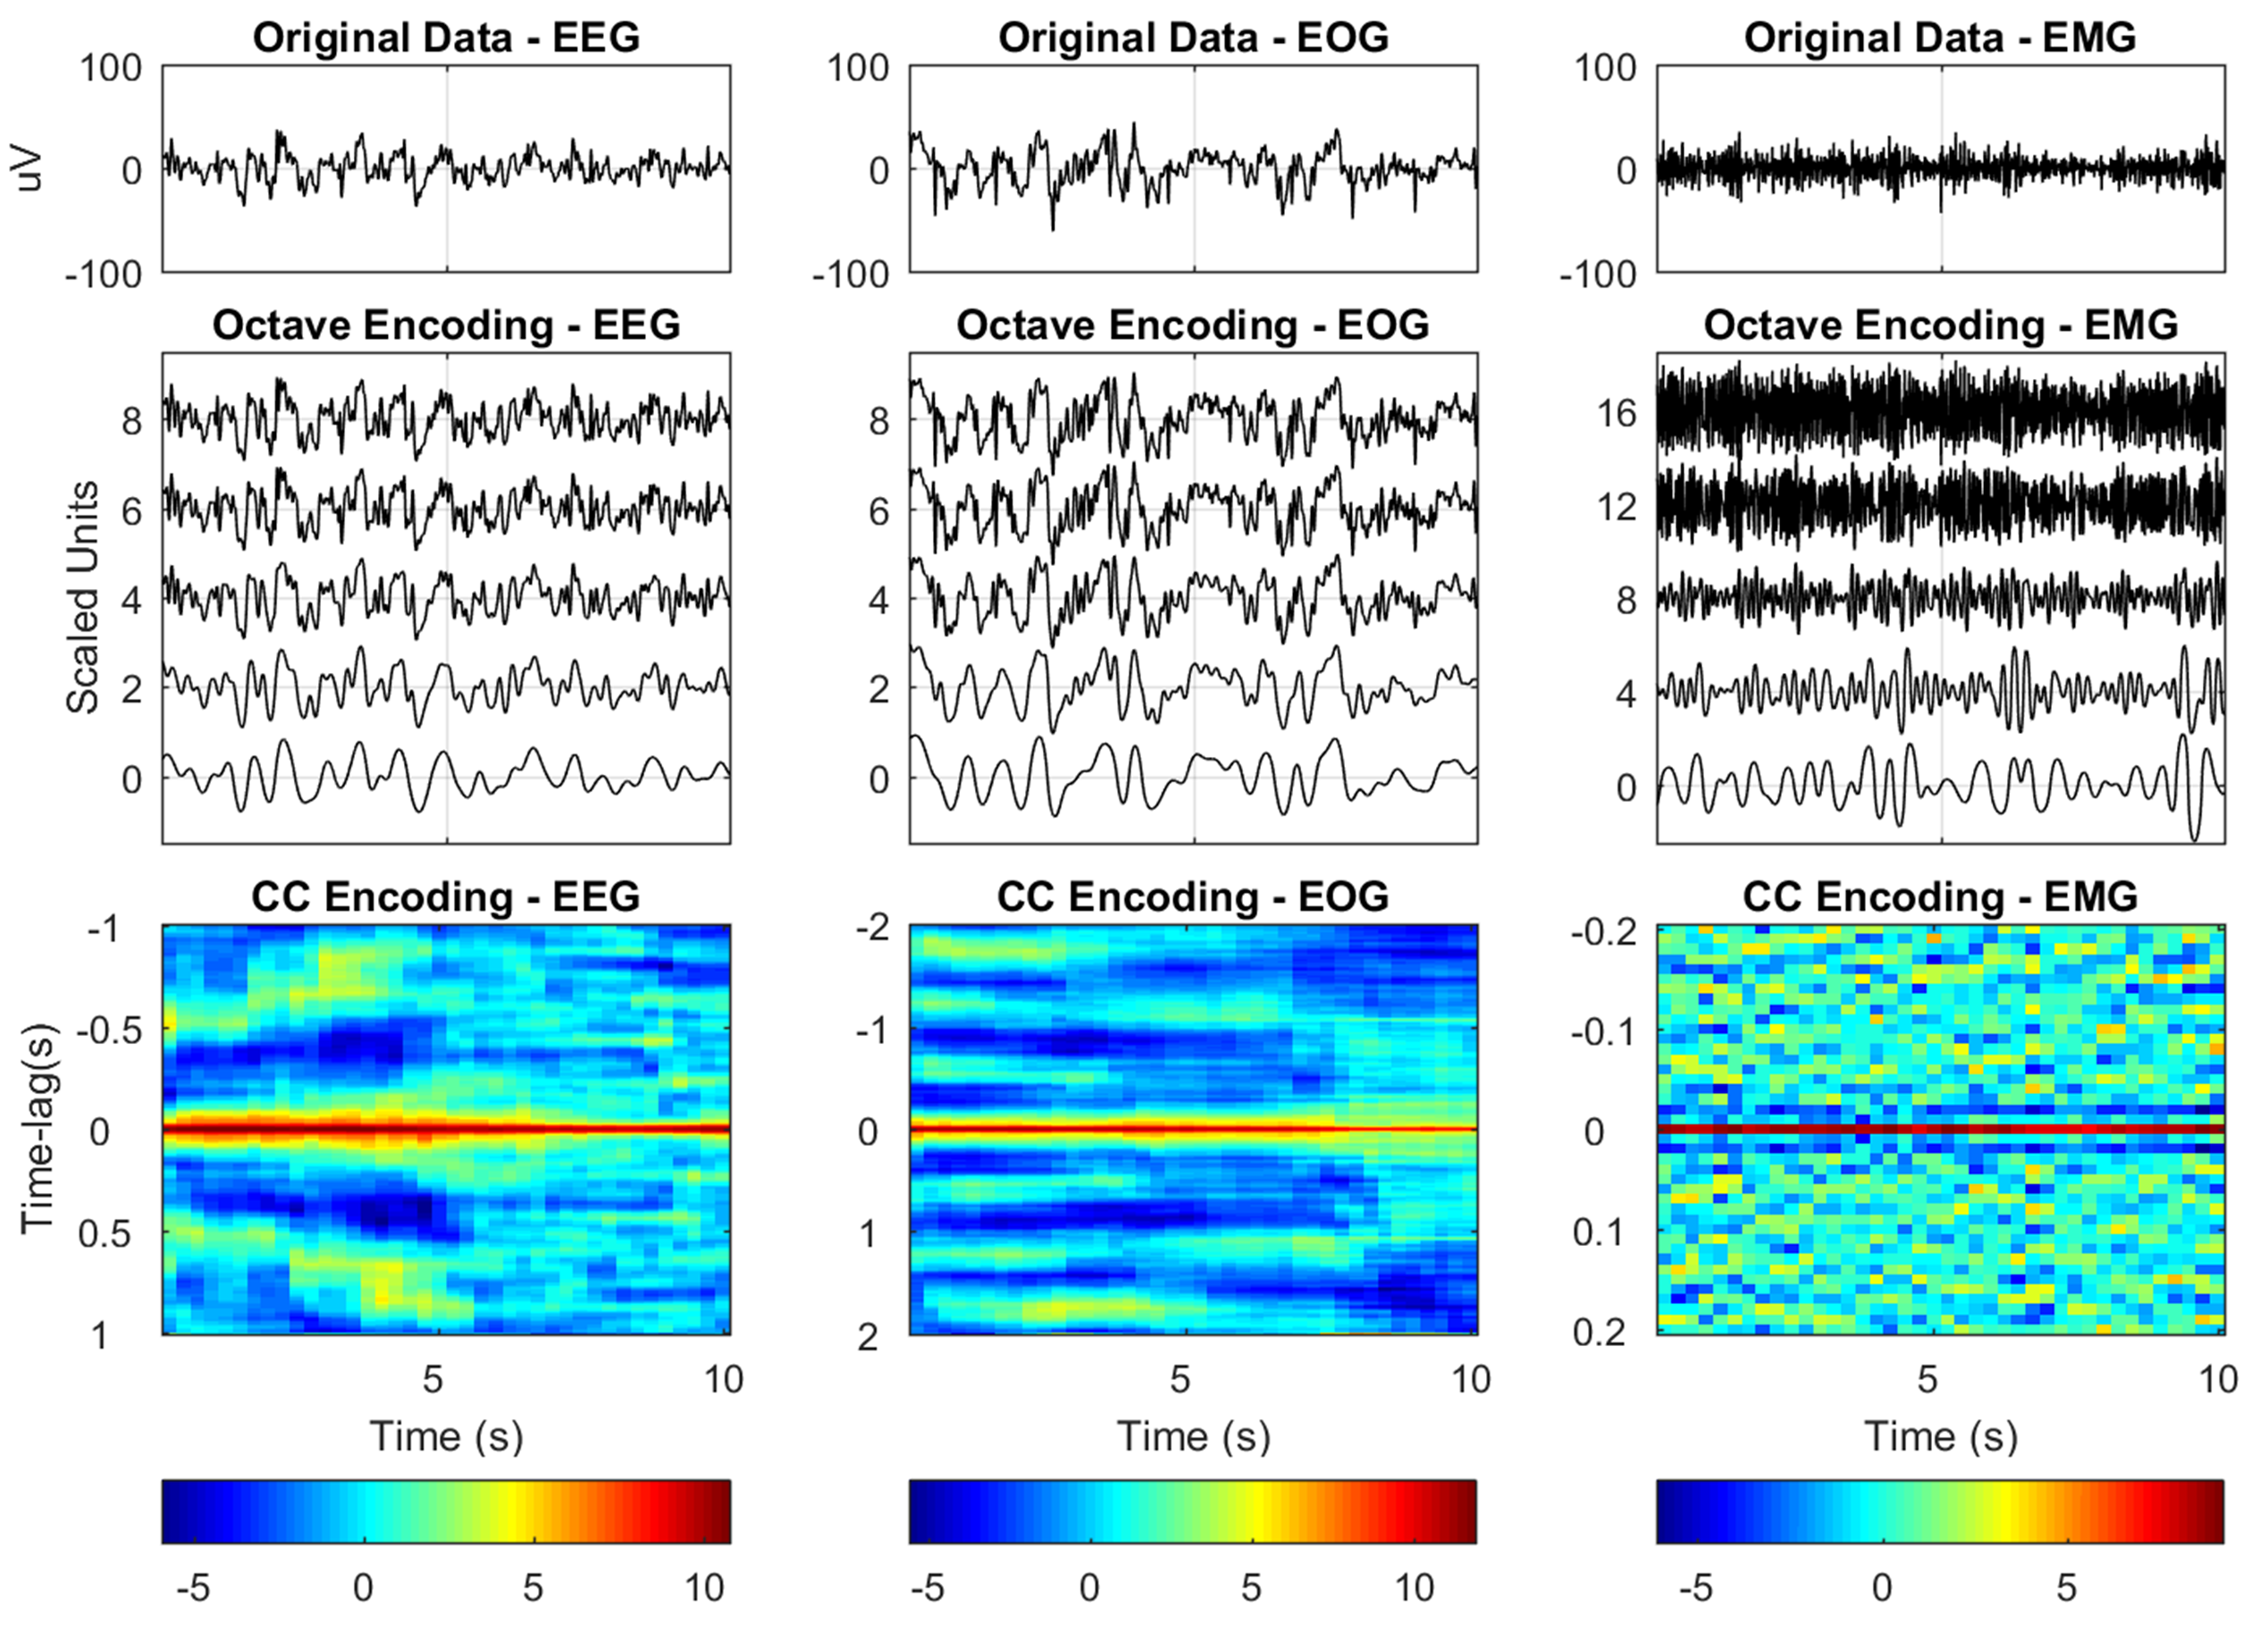
\includegraphics[width=\linewidth]{figures/paper-iii/ncomm_figure6a-2}}  \\
    \subfloat[]
    {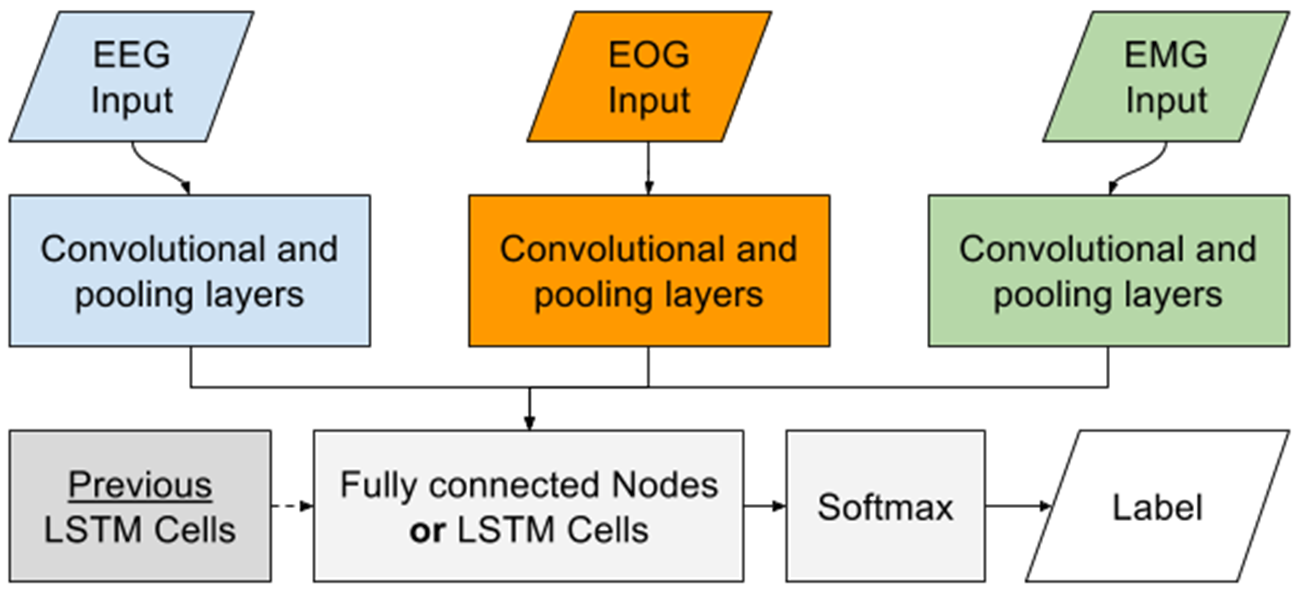
\includegraphics[width=0.7\linewidth]{figures/paper-iii/ncomm_figure6b-2}}
    \caption[Neural network strategy for \acs{STAGES} model]{Neural network strategy for \ac{STAGES} model. (a) An example of the octave and the \ac{CC} encoding on 10 s of \ac{EEG}, \ac{EOG} and \ac{EMG} data. These processed data are fed into the neural networks in one of the two formats. The data in the octave encoding are offset for visualization purposes. Color scale is unitless. (b) Simplified network configuration, displaying how data are fed and processed through the networks. A more detailed description of the network architecture is shown in~\cref{fig:sleep-stages:paper-iii:figure-s03}.}
    \label{fig:sleep-stages:paper-iii:figure-06}
\end{adjustwidth*}
\end{figure}

Octave encoding maintains all information in the signal, and enriches it by repeatedly removing the top half of the bandwidth (i.e. cut off frequencies of \SIlist{49;25;12.5;6.25;3.125}{\hertz}) using a series of low-pass filters, yielding a total of 5 new channels for each original channel. 
At no point is a high-pass filter applied. 
Instead, the high frequency information may be obtained by subtracting lower frequency channels---an association the neural networks can make, given their universal approximator properties~\cite{Hornik1989}. 
After filtration, each new channel is scaled to the \nth{95} percentile and log modulus transformed:
\begin{equation}
    \mathbf{x}_{\mathrm{scaled}} = \sign \parentheses*{ \mathbf{x} } \log \parentheses*{\frac{|\mathbf{x}|}{p_{95}(\mathbf{x})} + 1 }
\end{equation}
The initial scaling places \nth{95} of the data between -1 and 1, a range in which the log modulus is close to linear. 
Very large values, such as those found in particularly noisy areas, are attenuated greatly. 
Some recordings are noisy, making the \nth{95} percentile significantly higher than what the physiology reflects. 
Therefore, instead of the selecting the \nth{95} percentile from the entire recording, the recording is separated into 50\% overlapping \SI{90}{\minute} segments, from which the \nth{95}th percentile is computed. 
The mode of these values is then used as a scaling reference. 
In general, scaling and normalization is important to ensure quick convergence as well as generalization in neural networks. 
The decomposition is done in the same way on every channel, resulting in 25 new channels in total.

\begin{figure}
\begin{adjustwidth*}{}{-\marginparwidth-\marginparsep}
    \centering
    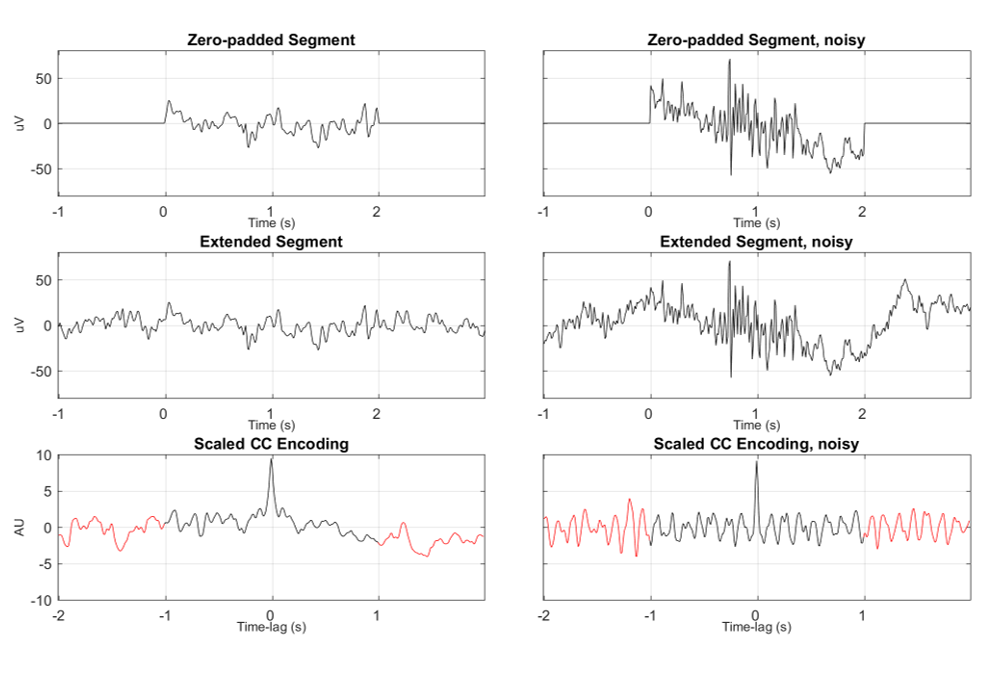
\includegraphics[width=\linewidth]{figures/paper-iii/SuppFigure_5.png}
    \caption[\acs{CC} encoding example]{Implementation of \acs{CC} encoding. \ac{CC} encoding of a noisy (right) and less noisy (left) signal. The central part of the encoding, representing areas of full overlap between correlated signals, is kept; the red part is discarded.}
    \label{fig:sleep-stages:paper-iii:figure-s05}
\end{adjustwidth*}
\end{figure}

Using a \ac{CC} function, underlying periodicities in the data are revealed while noise is attenuated. 
White noise is by definition uncorrelated; the auto-correlation function is zero everywhere except in lag zero. 
It is this property that is utilized, even though noise cannot always be modeled as such. 
\ac{PSG} signals are often obscured by undesired noise that is uncorrelated with other aspects of the signals. 
An example \ac{CC} between a signal segment and an augmented version of the same signal segment is shown in~\cref{fig:sleep-stages:paper-iii:figure-s05}. 

Choosing the \ac{CC} in this manner over a standard auto-correlation function serves two purposes: the slow frequencies are expressed better, since there is always full overlap between the two signals\graffito{Although some of this can be adjusted with the normal auto-correlation function using an unbiased estimate.}; and the change in fluctuations over time within a segment is expressed, making the function reflect aspects of stationarity. 
Because this is the \ac{CC} between a signal and an augmented version of itself, the zero lag represents the power of that segment, as is the case in an auto-correlation function.

Frequency content with a time resolution may also be expressed using time-frequency decompositions, such as spectrograms or scalograms.
One of the key properties of a \ac{CNN}, however, is the ability to detect distinct features anywhere in an input given the latent property of equivariance~\cite{Lenc2015}. 
A \ac{CC} function reveals an underlying set of frequencies as an oscillation pattern, as opposed to a spectrogram, where frequencies are displayed as small streaks or spots in specific locations, corresponding to time-specific frequencies.
The length and size of each \ac{CC} reflects the expected frequency content and the limit of quasi-stationarity\graffito{That is, how quickly the frequency content is expected to change.}.

The \ac{EEG} signal is quasi-stationary in signals with a length of up to \SI{0.25}{\second}~\cite{Amzica1998,Kaplan2005}.
The lowest expected meaningful frequencies are delta rhythms, which have a lower bound of 0.5 Hz~\cite{Amzica1998}. 
Hence, the transformation is made up of \SI{2}{\second} segments with \SI{1.75}{\second} overlaps between segments.

The \ac{EOG} signal reveals information about eye movements such as \acp{REM}, and to some extent \ac{EEG} activity~\cite{Malhotra2014, Berry2017}. 
In the case of the \ac{EOG} signal, the relative phase between the two channels is of great importance to determine synchronized eye movements, and hence a \ac{CC} of opposite channels\graffito{Either the augmented or zero-padded signal is replaced with the opposite channel.} is also included. 
The slowest eye-movements happen over the course of several seconds~\cite{Malhotra2014, Berry2017}, and hence a segment length of \SI{4}{\second} was selected for the correlation functions. 
To maintain resolution flexibility with the \ac{EEG}, an overlap of \SI{3.75}{\second} between each data segment was selected.

In the case of the \ac{EMG} signal, the main concern is the signal amplitude and the temporal resolution, not the actual frequencies. As no relevant low frequency content is expected, a segment length of 0.4 seconds and an overlap of 0.25 seconds was selected.

As with the octave encoding, the data is scaled, although only within segments:

\begin{equation}
    D_i = \frac{ \gamma_{\mathbf{x}_i \mathbf{y}_i} \func{\log}{1 + \max \abs*{\gamma_{\mathbf{x}_i \mathbf{y}_i}}}}{\max \abs*{\gamma_{\mathbf{x}_i \mathbf{y}_i}}}
\end{equation}
where $D_i$ is the scaled correlation function and $\gamma_{\mathbf{x}_i \mathbf{y}_i}$ is the unscaled correlation function.

\subsubsection{Architectures of applied \ac{CNN} models}

\begin{figure}
\begin{adjustwidth*}{}{-\marginparwidth-\marginparsep}
    \centering
    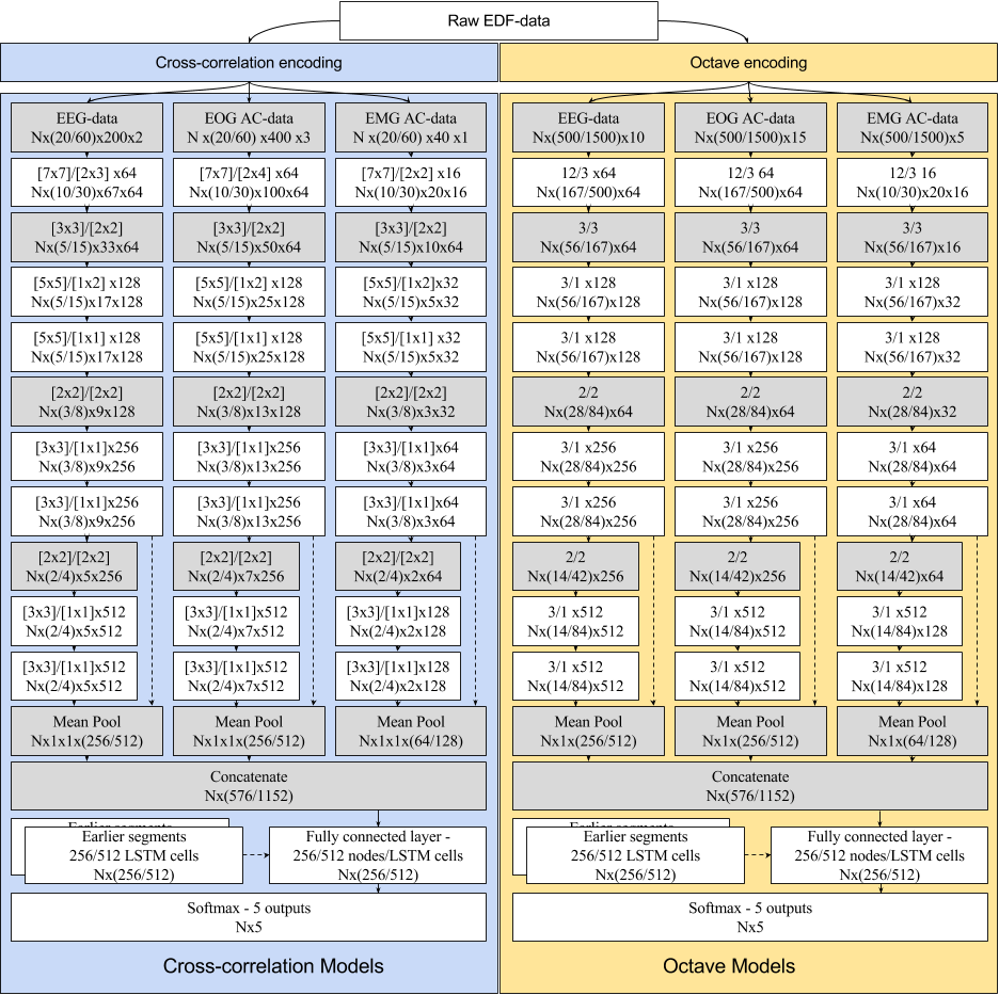
\includegraphics[width=\linewidth]{figures/paper-iii/SuppFigure_3.png}
    \caption[Network configurations]{Specifications of each network configuration. Each block represents an operation; white blocks require multiplications and additions, whereas grey blocks are pooling or concatenations, default being maximum pooling. The top row of each block describes the size of the window and its stride, and the bottom row describes the size of the output. In this output, \(N\) is the length of a sequence, the second dimension is the segment length, and if a fourth dimension is present (\acs{CC} models), the third dimension originally represents the size of the correlation function. The last dimension is the number of features in that layer. Models with a low complexity skip the third max pooling block, and go straight to mean pooling.}
    \label{fig:sleep-stages:paper-iii:figure-s03}
\end{adjustwidth*}
\end{figure}

The architecture of a \ac{CNN} typically reflects the complexity of the problem that is being solved and how much training data is available, as a complex model has more parameters than a simple model and is therefore more likely to overfit.
However, much of this may be solved using proper regularization. 
Another restriction is the resources required to train a model; deep and complex models require far more operations and will therefore take longer to train and operate. 
In this study, no exhaustive hyper-parameter optimization was carried out. 
The applied architectures were chosen on the basis of other published models~\cite{Simonyan2015}. 
Since the models utilized three separate modalities (\ac{EEG}, \ac{EOG} and \ac{EMG}), three separate sub-networks were constructed. 
These were followed by fully connected layers combining the inputs from each sub-network, which were passed onto a softmax output, as shown in~\cref{fig:sleep-stages:paper-iii:figure-06}b and~\cref{fig:sleep-stages:paper-iii:figure-s03}. 
Models that utilize memory have fully connected hidden units replaced with \ac{LSTM} cells and recurrent connections added between successive segments. 
Networks of two different sizes are evaluated to quantify the effect of increasing complexity. 

\subsubsection{Training of \ac{CNN} models}
Training the models involves optimizing parameters to minimize a loss function evaluated across a training dataset.
The loss function was defined as the cross-entropy with \(\ell_2\) regularization:
\begin{align}
\begin{split}
    \func{L}{\boldsymbol{\omega}} &= \frac{1}{N}\sum_{i=1}^{N} \func{H}{\mathbf{y}_i, \hat{\mathbf{y}}_i} + \ell_2 \\
    &= \frac{1}{N}_{i=1}^{N} \mathbf{y}_i \func{\log}{\hat{\mathbf{y}}_i} + \parentheses*{ 1 - \mathbf{y}_i } \func{\log}{1 - \hat{\mathbf{y}}_i} + \lambda \| \boldsymbol{\omega} \|^2_2,
\end{split}
\end{align}
where $\mathbf{y}_i$ is the true class label of the \textit{i}th window, $\hat{\mathbf{y}}_i$ is the estimated probability of the \textit{i}th window, $\omega$ is the parameter to be updated, and $\lambda$ is the weight decay parameter set at $10^{-5}$. 
The model parameters were initialized with $\func{\mathcal{N}}{0, 0.01}$, and trained until convergence using stochastic gradient decent with momentum~\cite{Polyak1964}. 
Weight updates were computed as: 
\begin{align}
    \boldsymbol{\omega}_{t+1} &= \boldsymbol{\omega}_t + \eta \mathbf{v}_{t+1} \\
    \mathbf{v}_{t+1} &= \alpha \mathbf{v}_t - \frac{\partial \mathbf{L}}{\partial \boldsymbol{\omega}_t},
\end{align}
where $\alpha$ is the momentum set at 0.9, $\mathbf{v}_t$ is the learning velocity initialized at 0, and $\eta$ is the learning rate, initially set at 0.005. 
The learning rate was gradually reduced with an exponential decay 
\begin{equation}
    \eta = \eta_0 \exp \parentheses*{-t/\tau},
\end{equation}
where $t$ is the number of updates and $\tau$ is a time constant, here set to \num{12000}.

Over-fitting was avoided using a number of regularization techniques, including batch normalization~\cite{Ioffe2015}, weight decay~\cite{Krogh1992}, and early stopping~\cite{Caruana2000}. 
Early stopping is accomplished by scheduling validation after every \nth{50} training batch. 
This is done by setting aside 10\% of the training data.
Training is stopped if the validation accuracy starts to decrease as a sign of over-fitting. 
For \ac{LSTM} networks, dropout set at 0.50 was included while training~\cite{Srivastava2014}.
This ensured that model parameters generalized to the validation data and beyond.
Given the stochastic nature of the training procedure, it was likely that two realizations of the same model would not lead to the same results, since models end up in different local minima. 
To measure the effect of this, two realizations were made of each model.

Apart from model realizations, we also investigated the effect of ensembling our sleep stage classification model. 
In general, ensemble models can yield higher predictive performance than any single model by attacking a classification or regression problem from multiple angles. 
For our specific use case, this resolves into forming a sleep stage prediction based on the predictions of all the models in the given ensemble. 
We tested several ensembles containing various numbers of model architectures and data encodings, as described in~\cref{tab:sleep-stages:paper-iii:table-s08a,tab:sleep-stages:paper-iii:table-s08b}. 

\subsubsection{Performance comparisons of generated \ac{CNN} models}
As stated, the influences of many different factors were analyzed. 
These included: using octave or \ac{CC} encoding, short (\SI{5}{\second}) or long (\SI{15}{\second}) segment lengths, low or high complexity, with or without \ac{LSTM}, and using only a single or two realizations of a given model. 
To quantify the effect of each in a principled manner, a $2^5$-factorial experiment was designed leading to 32 different models as detailed in~\cref{tab:sleep-stages:paper-iii:table-s08a,tab:sleep-stages:paper-iii:table-s08b}.
Comparisons between models was done on a per epoch basis. 
% \begin{table}[tb]
%     \centering
%     \small
%     \caption[\acs{STAGES} models]{\ac{STAGES} model tested. 32 single models are tested, and 9 ensembles, totaling 41 models.}
%     \label{tab:sleep-stages:paper-iii:table-s08}
%     \begin{tabular}{@{}lllll@{}}
%         \toprule
%         \multicolumn{5}{c}{Single models} \\ \midrule
%         Memory        & Seg. Len. & Complexity & Encoding & Realizations \\
%         Simple FF     & 5 s       & Low        & Octave   & 1            \\
%         \ac{LSTM}          & 15 s      & High       & \ac{CC}       & 2            \\ \bottomrule
%     \end{tabular}
%     \\
%     \small
%     \begin{tabular}{@{}llllllllll@{}}
%         \toprule
%         \multicolumn{10}{c}{Ensembles} \\ \midrule
%         Parameters included & All Oct FF & All Oct \ac{LSTM} & All \ac{CC} FF & All \ac{CC} \ac{LSTM} & All FF & All \ac{LSTM} & All Oct models & All \ac{CC} models & All models \\
%         N. models           & 8          & 8            & 8         & 8           & 16     & 16       & 16             & 16            & 32         \\ \bottomrule
%     \end{tabular}
% \end{table}

\begin{table}[tb]
    \centering
    \small
    \caption[Experimental configurations for single models]{Experimental configurations for single models}
    \label{tab:sleep-stages:paper-iii:table-s08a}
    \begin{tabular}{@{}llllll@{}} \toprule
        \textbf{Level} & \textbf{Memory} & \textbf{Segment duration} & \textbf{Complexity} & \textbf{Encoding} & \textbf{Realizations} \\ \midrule
        1 & Simple \acs{FF} & \SI{5}{\second} & Low & Octave & 1 \\
        2 & \acs{LSTM} & \SI{15}{\second} & High & \acs{CC} & 2 \\ \bottomrule
    \end{tabular}
\end{table}

\begin{table}[tb]
\begin{adjustwidth*}{}{-\marginparwidth-\marginparsep}
    % \centering
    \small
    \caption[Experimental configurations for ensemble models]{Experimental configurations for ensemble models}
    \label{tab:sleep-stages:paper-iii:table-s08b}
    \begin{tabular}{@{}llllllllll@{}} \toprule
        \textbf{Configuration} & Oct FF & Oct \ac{LSTM} & \ac{CC} FF & \ac{CC} \ac{LSTM} & FF & \ac{LSTM} & Oct & \ac{CC} & All models \\
        \textbf{Number of models} & 8 & 8 & 8 & 8 & 16 & 16 & 16 & 16 & 32 \\ \bottomrule
    \end{tabular}
\end{adjustwidth*}
\end{table}

% \begin{landscape}
\begin{table}[t]
\begin{adjustwidth*}{}{-\marginparwidth-\marginparsep}
\begin{threeparttable}
    \small
    \centering
    \caption[\acs{IS-RC} model performance]{Individual and overall scorer performance compared to model performance on \ac{IS-RC} data.}
    \label{tab:sleep-stages:paper-iii:table-01}
    \begin{tabular}{@{}llllllll@{}}
        \toprule
                                           & \textbf{Overall}      &\textbf{ Scorer 1 }              &\textbf{ Scorer 2   }            & \textbf{Scorer 3}                & \textbf{Scorer 4  }            & \textbf{Scorer 5}               & \textbf{Scorer 6}                \\ \midrule
        \textbf{Accuracy, \%}                       &              &                        &                        &                         &                       &                        &                         \\
        \quad Biased                       & $81.3\pm3.0$ & $82.4\pm6.1$           & $84.6\pm5.5$           & $74.1\pm7.9$            & $85.4\pm5.7$          & $83.1\pm9.4$           & $78.3\pm8.9$            \\
        \quad Unbiased                     & $76.0\pm3.2$ & $77.3\pm6.3$           & $79.1\pm6.3$           & $69.0\pm8.0$            & $79.7\pm6.5$          & $77.8\pm9.6$           & $72.9\pm9.2$            \\
        \quad Model, \%                    & -            & $85.1\pm4.9$           & $83.8\pm5.0$           & $86.5\pm4.3$            & $84.3\pm4.7$          & $85.6\pm4.7$           & $87.0\pm4.5$            \\
        \textit{p}-value & -            & $3.8 \times 10^{-14}$ & $7.5\times 10^{-9}$  & $6.0\times10^{-28}$ & $4.7\times10^{-9}$ & $1.7\times10^{-8}$  & $7.5\times10^{-19}$ \\ \midrule
        \textbf{\cohen}                             &              &                        &                        &                         &                       &                        &                         \\
        \quad Biased                       & $61.0\pm6.8$ & $63.6\pm12.2$          & $68.4\pm10.5$          & $45.6\pm19.7$           & $69.6\pm13.2$         & $64.5\pm20.9$          & $54.5\pm19.8$           \\
        \quad Unbiased                     & $57.7\pm6.1$ & $61.3\pm11.2$          & $64.6\pm10.3$          & $43.5\pm19.2$           & $64.6\pm13.1$         & $60.9\pm16.9$          & $51.6\pm16.7$           \\
        \quad Model                        & -            & $74.3\pm12.3$          & $72.4\pm12.1$          & $76.0\pm11.8$           & $72.7\pm12.0$         & $74.7\pm12.1$          & $76.6\pm12.2$           \\
        \textit{p}-value & -            & $4.6\times10^{-14}$ & $7.9\times10^{-10}$ & $7.0\times10^{-24}$ & $6.4\times10^{-9}$ & $9.2\times10^{-10}$ & $2.0\times10^{-20}$ \\ \bottomrule
    \end{tabular}
    \begin{tablenotes}
    \small \item Both accuracy and \cohen are presented with (biased) and without (unbiased) the assessed scorer included in the consensus standard in a leave-one-out fashion. Accuracy is expressed in percent, and \cohen is a ratio and therefore unitless. \textit{p}-values correspond to the paired \textit{t}-tests between the unbiased predictions for each scorer against the model predictions on the same consensus.
    \end{tablenotes}
\end{threeparttable}
\end{adjustwidth*}
\end{table}
% \end{landscape}

% \begin{table}[tb]
% % \begin{adjustwidth*}{}{-\marginparwidth-\marginparsep}
%     \small
%     \centering
%     \caption[\acs{STAGES} model experimental configurations]{\ac{STAGES} model experimental configurations. 32 single models are tested, and 9 ensembles, totaling 41 models.}
%     \label{tab:sleep-stages:paper-iii:table-s08}
%     \begin{tabular}{@{}lllllllllll@{}}
%         \toprule
%         \multirow{3}{*}{Single models} & \multicolumn{2}{l}{Memory}        & \multicolumn{2}{l}{Seg. Len.} & \multicolumn{2}{l}{Complexity} & \multicolumn{2}{l}{Encoding} & \multicolumn{2}{l}{Realizations} \\ \midrule
%         & \multicolumn{2}{l}{Simple FF}     & \multicolumn{2}{l}{5 s}       &\multicolumn{2}{l}{Low}        & \multicolumn{2}{l}{Octave}   & \multicolumn{2}{l}{1}            \\
%         & \multicolumn{2}{l}{\ac{LSTM}}          & \multicolumn{2}{l}{15 s}      & \multicolumn{2}{l}{High}       & \multicolumn{2}{l}{\ac{CC}}       & \multicolumn{2}{l}{2}            \\ \midrule
%         \multirow{2}{*}{Ensemble models} & & Oct FF & Oct \ac{LSTM} & \ac{CC} FF & \ac{CC} \ac{LSTM} & FF & \ac{LSTM} & Oct & \ac{CC} & All models \\
%         & & 8          & 8            & 8         & 8           & 16     & 16       & 16             & 16            & 32         \\ \bottomrule
%     \end{tabular}
%     % \\
%     % \small
%     % \begin{tabular}{@{}llllllllll@{}}
%     %     \toprule
%     %     \multicolumn{10}{c}{Ensembles} \\ \midrule
%     %     Parameters included & All Oct FF & All Oct \ac{LSTM} & All \ac{CC} FF & All \ac{CC} \ac{LSTM} & All FF & All \ac{LSTM} & All Oct models & All \ac{CC} models & All models \\
%     %     N. models           & 8          & 8            & 8         & 8           & 16     & 16       & 16             & 16            & 32         \\ \bottomrule
%     % \end{tabular}
% % \end{adjustwidth*}
% \end{table}

\subsection{Results}
\subsubsection{Inter-scorer reliability cohort}

We assessed inter-scorer reliability using the \ac{IS-RC}, a cohort of 70 \acp{PSG} scored by 6 scorers across three locations in the USA~\cite{Kuna2013}.
\cref{tab:sleep-stages:paper-iii:table-01} displays individual scorer performance as well as the averaged performance across scorers, with top and bottom of table showing accuracies and \cohen, respectively.
The results are shown for each individual scorer when compared to the consensus of all scorers (biased), and compared to the consensus of the remaining scorers (unbiased).
In the event of no majority vote for an epoch, the epoch was counted equally in all classes in which there was disagreement.
Also shown in~\cref{tab:sleep-stages:paper-iii:table-01} is the model performance on the same consensus scorings as each individual scorer along with the \textit{t}-statistic and associated \textit{p}-value for each paired \textit{t}-test between the model performance and individual scorer performance. 
At a significance level of \(\alpha=0.05\), the model performs statistically better than any individual scorer both in terms of accuracy and \cohen.

% \begingroup
% \setlength{\tabcolsep}{0pt} % Default value: 6pt
\begin{table}[tb]
\small
\centering
\begin{threeparttable}
\caption[\acs{IS-RC} scorer assessment]{\acs{IS-RC} scorer assesment.}
\label{tab:sleep-stages:paper-iii:table-s02}
\begin{tabular}{@{}llSSSSSS@{}}
\toprule
    &        & \multicolumn{5}{c}{\textbf{Concensus}}                 &   \\ \cline{3-7}
    &  & \acs{W}    & \acs{N1}     & \acs{N2}      & \acs{N3}        & \acs{REM}     & Pr      \\ \midrule
    \multirow{10}{*}{\rotatebox[origin=c]{90}{\textbf{Individual scorers}}} & \acs{W}   & \cellcolor[HTML]{EFEFEF0}13.28 \% & 1.04 \% & 0.86 \%  & 0.08 \% & 0.23 \%  & 0.86 \\
    &           & \cellcolor[HTML]{EFEFEF0}13.25 \% & 0.98 \% & 0.87 \%  & 0.08 \% & 0.22 \%  & 0.86 \\
    & \acs{N1}  & 0.79 \% & \cellcolor[HTML]{EFEFEF0}3.36 \% & 1.23 \%  & 0.03 \% & 0.29 \%  & 0.59 \\
    &           & 0.88 \% & \cellcolor[HTML]{EFEFEF0}3.61 \% & 1.42 \%  & 0.03 \% & 0.31 \%  & 0.58 \\
    & \acs{N2}  & 0.87 \%  & 2.46 \% & \cellcolor[HTML]{EFEFEF0}44.66 \% & 4.89 \% & 0.85 \%  & 0.83 \\
    &           & 0.84 \%  & 2.30 \% & \cellcolor[HTML]{EFEFEF0}45.48 \% & 5.92 \% & 0.84 \%  & 0.82 \\
    & \acs{N3}  & 0.05 \%  & 0.02 \% & 2.58 \%  & \cellcolor[HTML]{EFEFEF0}6.45 \% & 0.00 \%  & 0.71 \\
    &           & 0.05 \%  & 0.02 \% & 1.54 \%  & \cellcolor[HTML]{EFEFEF0}5.41 \% & 0.00 \%  & 0.77 \\
    & \acs{REM} & 0.32 \%  & 1.00 \% & 1.14 \%  & 0.03 \% & \cellcolor[HTML]{EFEFEF0}13.46 \% & 0.84 \\
    &           & 0.31 \%  & 0.97 \% & 1.16 \%  & 0.04 \% & \cellcolor[HTML]{EFEFEF0}13.46 \% & 0.84 \\
    & Se        & 0.87    & 0.43   & 0.88    & 0.56   & 0.91    & 0.81 \\
    &           & 0.86    & 0.46   & 0.9     & 0.47   & 0.91    & 0.81 \\ \bottomrule
\end{tabular}
\begin{tablenotes}
\small \item %
\describe{W}; %
\describe{N1}; %
\describe{N2}; %
\describe{N3}; %
\describe{REM}; %
Pr, precision; Se, sensitivity.
\end{tablenotes}
\end{threeparttable}
\end{table}
% \endgroup

\cref{tab:sleep-stages:paper-iii:table-s02} displays the confusion matrix for every epoch of every scorer of the inter-scorer reliability data, both unadjusted (top) and adjusted (bottom).
As in~\cite{Rosenberg2013}, the biggest discrepancies occur between \ac{N1} and \ac{W}, \ac{N1} and \ac{N2}, and \ac{N2} and \ac{N3}, with some errors also occurring between \ac{N1} and \ac{REM}, and \ac{N2} and \ac{REM}.

For future analyses of the \ac{IS-RC} in combination with other cohorts that have been scored only by one scorer, a final hypnogram consensus was built for this cohort based on the majority vote weighted by the degree of consensus from each voter, expressed as 
\begin{equation}
    \text{\cohen}= 1 + \frac{1 - p_o}{1 - p_e},
\end{equation}
where $p_e$ is the baseline accuracy and $p_o$ is the scorer accuracy, such that
\begin{equation}
    \mathbf{y} = \argmax \frac{\sum_{i=1}^{6} \hat{\mathbf{y}}_i \cdot \boldsymbol{\kappa}_i}{\sum_{i=1}^{6} \boldsymbol{\kappa}_i}
\end{equation}
In this implementation, scorers with a higher consensus with the group are considered more reliable and have their assessments weighted heavier than the rest.
This also avoided split decisions on end-results.

\begin{table}[tb]
    % \centering
    \caption[\acs{STAGES} test performance]{Performance of best models on various datasets compared to the six-scorer consensus. All comparisons are on a by-epoch-basis.}
    \label{tab:sleep-stages:paper-iii:table-02}
    \small
    \begin{tabular}{@{}lllll@{}}
        \toprule
        \textbf{Test data}          & \textbf{Best single model} & \textbf{Accuracy, \%} & \textbf{Best ensemble} & \textbf{Accuracy}, \% \\ \midrule
        \ac{WSC}                & \ac{CC}/SH/LS/\ac{LSTM}/2   & $86.0 \pm 5.0$       & All \ac{CC}        & $86.4 \pm 5.2$       \\
        \ac{SSC}+\ac{KHC} & & & & \\
        \quad $\div$ narcolepsy            & \ac{CC}/LH/SS/\ac{LSTM}     & $76.9 \pm 11.1$      & All \ac{CC}        & $77.0 \pm 11.9$      \\
        \quad $+$ narcolepsy & \ac{CC}/LH/SS/\ac{LSTM}     & $68.8 \pm 11.0$      & All \ac{CC}        & $68.4 \pm 12.2$      \\
        \ac{IS-RC}              & \ac{CC}/LH/LS/\ac{LSTM}/2   & $84.6 \pm 4.6$       & All Models    & $86.8 \pm 4.3$       \\ \bottomrule
    \end{tabular}
\end{table}

\begin{figure}
\begin{adjustwidth*}{}{-\marginparwidth-\marginparsep}
    % \centering
    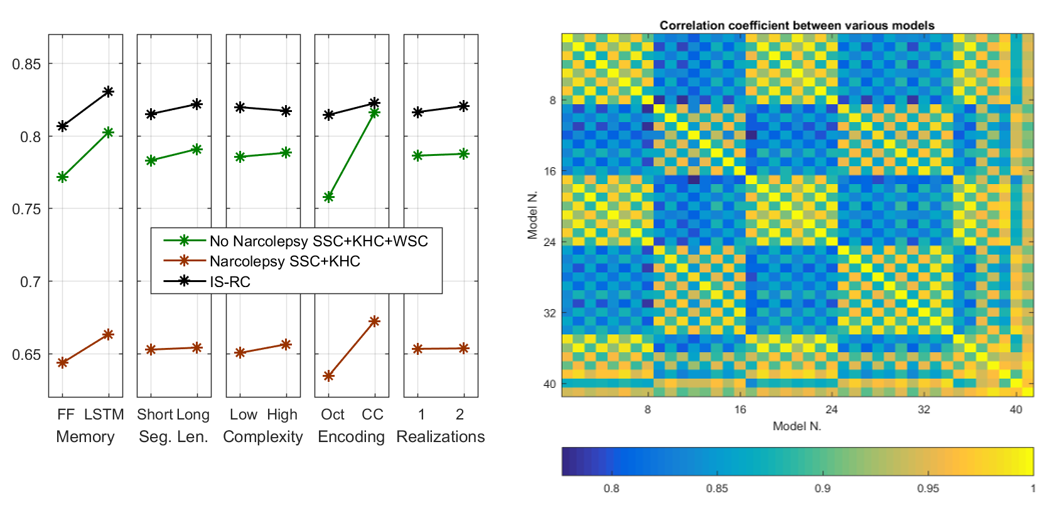
\includegraphics[width=\linewidth]{figures/paper-iii/SuppFigure_1.png}
    \caption[Comparisons of machine learning models]{Comparisons of machine learning models. Left: Comparisons of the effect on accuracy by each factor at different settings on \ac{IS-RC} data, \ac{SSC} and \ac{KHC} narcolepsy subjects, and the remaining \ac{SSC}, \ac{KHC} and \ac{WSC} subjects used for testing. Right: Correlation matrix showing similarities in different model predictions, where 0 means signals are independent, and 1 means signals are completely correlated. Models 1-32 are single models, and 33-41 are ensembles. The models vary on 5 parameters, each at two levels, in the following order: Memory – FF or \ac{LSTM}(1), segment size – 5 s or 15 s (2), complexity – high or low (3), encoding – \ac{CC} or octave (4), realizations – 1 or 2 (5). Ensembles: All FF octave models (33), all \ac{LSTM} octave models (34), all FF \ac{CC} models (35), all \ac{LSTM} \ac{CC} models (36), all FF models (37), all \ac{LSTM} models (38), all \ac{CC} models (39), all octave models (40), all models (41).}
    \label{fig:sleep-stages:paper-iii:figure-s01}
\end{adjustwidth*}
\end{figure}

\subsubsection{Optimizing machine learning performance for sleep staging}
We next explored how various machine learning algorithms (see Methods) performed depending on cohort, memory (i.e., feed forward (FF) versus \ac{LSTM} networks), signal segment length (short segments of 5 s (SS) versus long segments of 15 s (LS)), complexity (i.e., low (SH) vs. high (LH)), encoding (i.e., octave versus cross-correlation (\ac{CC}) encoding, and realization type (repeated training sessions).
The performance of these machine learning algorithms was compared with the six-scorer consensus in the \ac{IS-RC} and with single scorer data in 3 other cohorts, the Stanford Sleep Cohort (\ac{SSC})~\cite{Andlauer2013,Moore2014}, the Wisconsin Sleep Cohort (WSC)~\cite{Young2009,Moore2014} and the Korean Hypersomnia Cohort (\ac{KHC})~\cite{Hong2006,Andlauer2013} (see Datasets section in Methods for description of each cohort).

Model accuracy varies across datasets, reflecting the fact scorer performance may be different across sites, and because unusual subjects such as those with specific pathologies can be more difficult to score—a problem affecting both human and machine scoring. 
In this study, the worst performance was seen in the \ac{KHC} and \ac{SSC} with narcolepsy, and the best performance was achieved on \ac{IS-RC} data (\cref{fig:sleep-stages:paper-iii:figure-s01}a,~\cref{tab:sleep-stages:paper-iii:table-02}).
The \ac{SSC}+\ac{KHC} cohorts mainly contain patients with more fragmented sleeping patterns, which would explain a reduced performance. 
The \ac{IS-RC} has the most accurate label, minimizing the effects of erroneous scoring, which therefore leads to an increased performance.
Incorporating large ensembles of different models increased mean performances only slightly. (\cref{tab:sleep-stages:paper-iii:table-02}).

\begin{figure}[tb]
% \begin{adjustwidth*}{}{-\marginparwidth-\marginparsep}
    \centering
    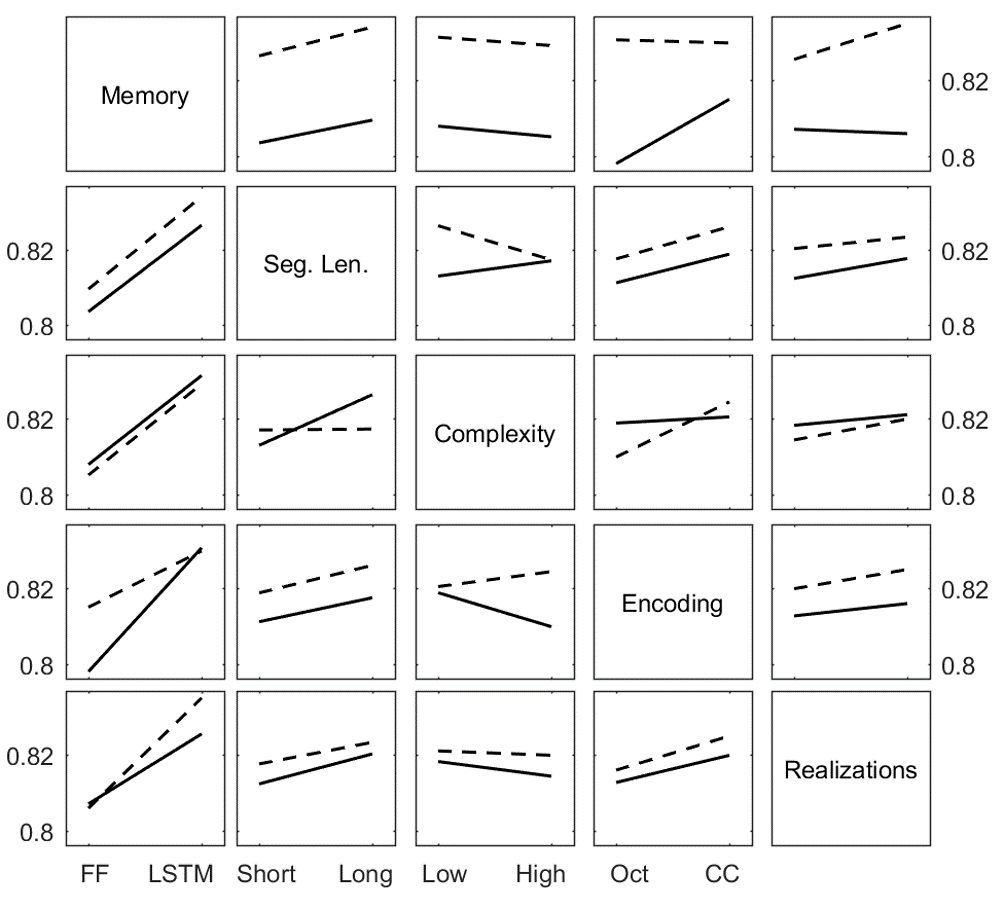
\includegraphics[width=\textwidth]{figures/paper-iii/SuppFigure_2.png}
    \caption[Factor interactions]{Interaction of different factors. The \ac{IS-RC} data was used for this analysis. The solid and dashed lines indicate factors along the rows on levels 1 and 2, respectively.}
    \label{fig:sleep-stages:paper-iii:figure-s02}
% \end{adjustwidth*}
\end{figure}

The two most important factors that increased prediction accuracy were encoding and memory, while segment length, complexity and number of realizations were less important (\cref{fig:sleep-stages:paper-iii:figure-s01}).
The effect of encoding was less prominent in the \ac{IS-RC}.
Prominent factor interactions include: (i) \ac{CC} encoding models improve with higher complexity, whereas octave encoding models worsen; (ii) increasing segment length positively affects models with low complexity, but does not affect models with a high complexity; and (iii) adding memory improves models with an octave encoding more than models with a \ac{CC} encoding.
Because the ISRC data are considered the most reliable, we decided to use these data as benchmark for model comparison.
This standard improved as more scorers were added, and the model performance increased (~\cref{fig:sleep-stages:paper-iii:figure-01}a).
The different model configurations described in this section do not represent exhaustive configuration search, and future work experiments might result in improved results.

\Cref{fig:sleep-stages:paper-iii:figure-02a} displays typical scoring outputs (bottom panels) obtained with a single sleep study of the \ac{IS-RC} cohort in comparison to 6 scorer consensus (top panel).
The model results are displayed as hypnodensity graphs, representing not only discrete sleep stage outputs, but also the probability of occurrence of each sleep state for each epoch (see definition in Data labels, scoring and fuzzy logic section).
As can be seen, all models performed well, and segments of the sleep study with the lowest scorer consensus (top) are paralleled by similar sleep stage probability uncertainty, with performance closest to scoring consensus achieved by an ensemble model described below (second to top).

\subsubsection{Final implementation of automatic sleep scoring algorithm}
Because of model noise, potential inaccuracies and the desire to quantify uncertainty, the final implementation of our sleep
scoring algorithm is an ensemble of different \ac{CC} models with
small variations in model parameters, such as the number of
feature-maps and hidden nodes.
This was achieved by randomly varying the parameters between 50 and 150\% of the original values using the \ac{CC}/SH/LS/\ac{LSTM} as a template (this model achieved similar performance to the \ac{CC}/LH/LS/\ac{LSTM} while requiring significantly less computational power).

% All models make errors, but as these errors occur independently of each other, the risk of not detecting and correcting errors falls with increasing model numbers.
% For this reason, 16 such models were trained, and at each analyzed segment both mean and variance of model estimates were calculated. 
We trained 16 models, and at each segment (\SIlist{5;10;15;30}{\second}) the mean and variance of model estimates were calculated. 
As expected, the relative model variance (standardized to the average variance in a correct wakefulness prediction) is generally lower in correct predictions and this can be used to inform users about uncertain/incorrect estimates. 
To demonstrate the effectiveness of this final implementation, the average of the models is shown alongside the distribution of \plusminus{5234}{14} scorers on 150 epochs, a dataset provided by the AASM (AASM inter-scorer reliability (ISR) dataset, (see Datasets section in Methods). 
On these epochs, the AASM ISR achieved a 90\% agreement between scorers. 
In comparison, the model estimates reached a 95\% accuracy compared to the AASM consensus (Fig. 2b). 
Using the model ensemble and reporting on sleep stage probabilities and inter-model variance for quality purpose constitute the core of our sleep scoring algorithm.
\begin{table}
% \begin{adjustwidth*}{}{-\marginparwidth-\marginparsep}
    \centering
    \small
\begin{threeparttable}
    \caption[\acs{STAGES} model confusion matrix]{Confusion matrix displaying the relation between different targets and the ensemble estimate.}
    \label{tab:sleep-stages:paper-iii:table-03}
    \begin{tabular}{@{}llSSSSSS@{}}
        \toprule
        &        & \multicolumn{5}{c}{\textbf{Target}}                    & \multicolumn{1}{l}{} \\ \cline{3-7}
        &  & \ac{W}    & \ac{N1}     & \ac{N2}      & \ac{N3}     & \ac{REM}     & Pr            \\ \midrule
        \multirow{10}{*}{\rotatebox[origin=c]{90}{\textbf{Model prediction}}} & \ac{W}   & \cellcolor[HTML]{EFEFEF0}14.08\% & 0.35\% & 0.88\%  & 0.01\% & 0.08\%  & 0.91                 \\
        &        & \cellcolor[HTML]{EFEFEF0}16.68\% & 0.15\% & 0.44\%  & 0.00\% & 0.02\%  & 0.96                 \\
        & \ac{N1}     & 1.13\%  & \cellcolor[HTML]{EFEFEF0}1.78\% & 3.00\%  & 0.00\% & 0.36\%  & 0.28                 \\
        &        & 0.47\%  & \cellcolor[HTML]{EFEFEF0}0.88\% & 1.15\%  & 0\%    & 0.12\%  & 0.34                 \\
        & \ac{N2}     & 0.29\%  & 0.59\% & \cellcolor[HTML]{EFEFEF0}52.58\% & 1.27\% & 0.66\%  & 0.95                 \\
        &        & 0.12\%  & 0.25\% & \cellcolor[HTML]{EFEFEF0}56.30\% & 0.34\% & 0.32\%  & 0.98                 \\
        & \ac{N3}     & 0.00\%  & 0\%    & 2.13\%  & \cellcolor[HTML]{EFEFEF0}4.87\% & 0\%     & 0.7                  \\
        &        & 0\%     & 0\%    & 1.09\%  & \cellcolor[HTML]{EFEFEF0}4.23\% & 0\%     & 0.91                 \\
        & \ac{REM}    & 0.54\%  & 1.17\% & 0.78\%  & 0\%    & \cellcolor[HTML]{EFEFEF0}13.45\% & 0.84                 \\
        &        & 0.40\%  & 0.73\% & 0.41\%  & 0\%    & \cellcolor[HTML]{EFEFEF0}15.86\% & 0.91                 \\
        & Se       & 0.88    & 0.46   & 0.89    & 0.79   & 0.92    & \cellcolor[HTML]{EFEFEF0}0.87                 \\
        &        & 0.94    & 0.44   & 0.95    & 0.92   & 0.97    & \cellcolor[HTML]{EFEFEF0}0.94                 \\ \bottomrule
    \end{tabular}
    \begin{tablenotes}
    \small \item Top row: unweighted consensus. Bottom row: weighted by the scorer agreement at each epoch. The number of analyzed epochs were \num{53009} (un-weighted) and \num{36032} (weighted). %
    \describe{W}; %
    \describe{N1}; %
    \describe{N2}; %
    \describe{N3}; %
    \describe{REM}; %
    Pr, precision; Se, sensitivity.
    \end{tablenotes}
\end{threeparttable}
% \end{adjustwidth*}
\end{table}
\subsubsection{Ensemble/best model performance}
\Cref{tab:sleep-stages:paper-iii:table-s02} reports on concordance for our best model, the ensemble of all \ac{CC} models.
Concordance is presented in a weighted and unweighted manner, between the best model estimate and scorer consensus (\cref{tab:sleep-stages:paper-iii:table-03}).
Weighing of a segment was based on scorer confidence and serves to weigh down controversial segments.
For each recording \textit{i}, the epoch-specific weight $w_n$ and weighted accuracy $\alpha w$ were calculated as:
\begin{align}
\begin{split}
    w_n &= \func{\max_{z \in \mathcal{Z}}}{\func{\mathbf{P}}{\mathbf{y}_n \mid \mathbf{x}_n}} - \func{\ell_{\mathcal{Z}}^2}{\func{\mathbf{P}}{\mathbf{y}_n \mid \mathbf{x}_n}}, \\
    \alpha_w^{(i)} &= \frac{1}{\sum_{\mathclap{n}} w_n} \sum_n w_n \parentheses*{ \func{\argmax_{m \in \mathcal{M}}}{\func{\mathbf{P}_m}{\hat{\mathbf{y}}_n | \mathbf{x}_n}} \cap \func{\argmax_{z \in \mathcal{Z}}}{\func{\mathbf{P}_z}{\mathbf{y}_n | \mathbf{x}_n}} },
\end{split}
\end{align}
where $\func{\ell_{\mathcal{Z}}^2}{\func{\mathbf{P}}{\mathbf{y}_n \mid \mathbf{x}_n}}$ is the second most likely stage assessed by the set of scorers (experts) denoted by $\mathcal{Z}$, of the \textit{n}th epoch in a sleep recording.
As with scorers, the biggest discrepancies occurred between wake versus \ac{N1}, \ac{N1} versus \ac{N2} and \ac{N2} versus \ac{N3}.
Additionally, the weighted performance was almost universally better than the unweighted performance, raising overall accuracy from 87 to 94\%, indicating a high consensus between automatic scoring and scorers in places with high scorer confidence.
An explanation for these results could be that both scorers and model are forced to make a choice between two stages when data are ambiguous.
An example of this may be seen in Fig. 2a.
Between 1 and 3 h, several bouts of \ac{N3} occur, although they often do not reach the threshold for being the most likely stage
As time progresses, more evidence for \ac{N3} appears reflecting increased proportion of slow waves per epoch, and confidence increases, which finally yields “definitive” \ac{N3}. 
This is seen in both model and scorer estimates.
Choosing to present the data as hypnodensity graphs mitigates this problem. 
The various model estimates produce similar results, which also resemble the scorer assessment distribution, although models without memory fluctuate slightly more, and tend to place a higher probability on \ac{REM} sleep in periods of wakefulness, since no contextual information is provided

\begin{figure}[p]
\begin{adjustwidth*}{}{-\marginparsep-\marginparwidth}
    % \centering
    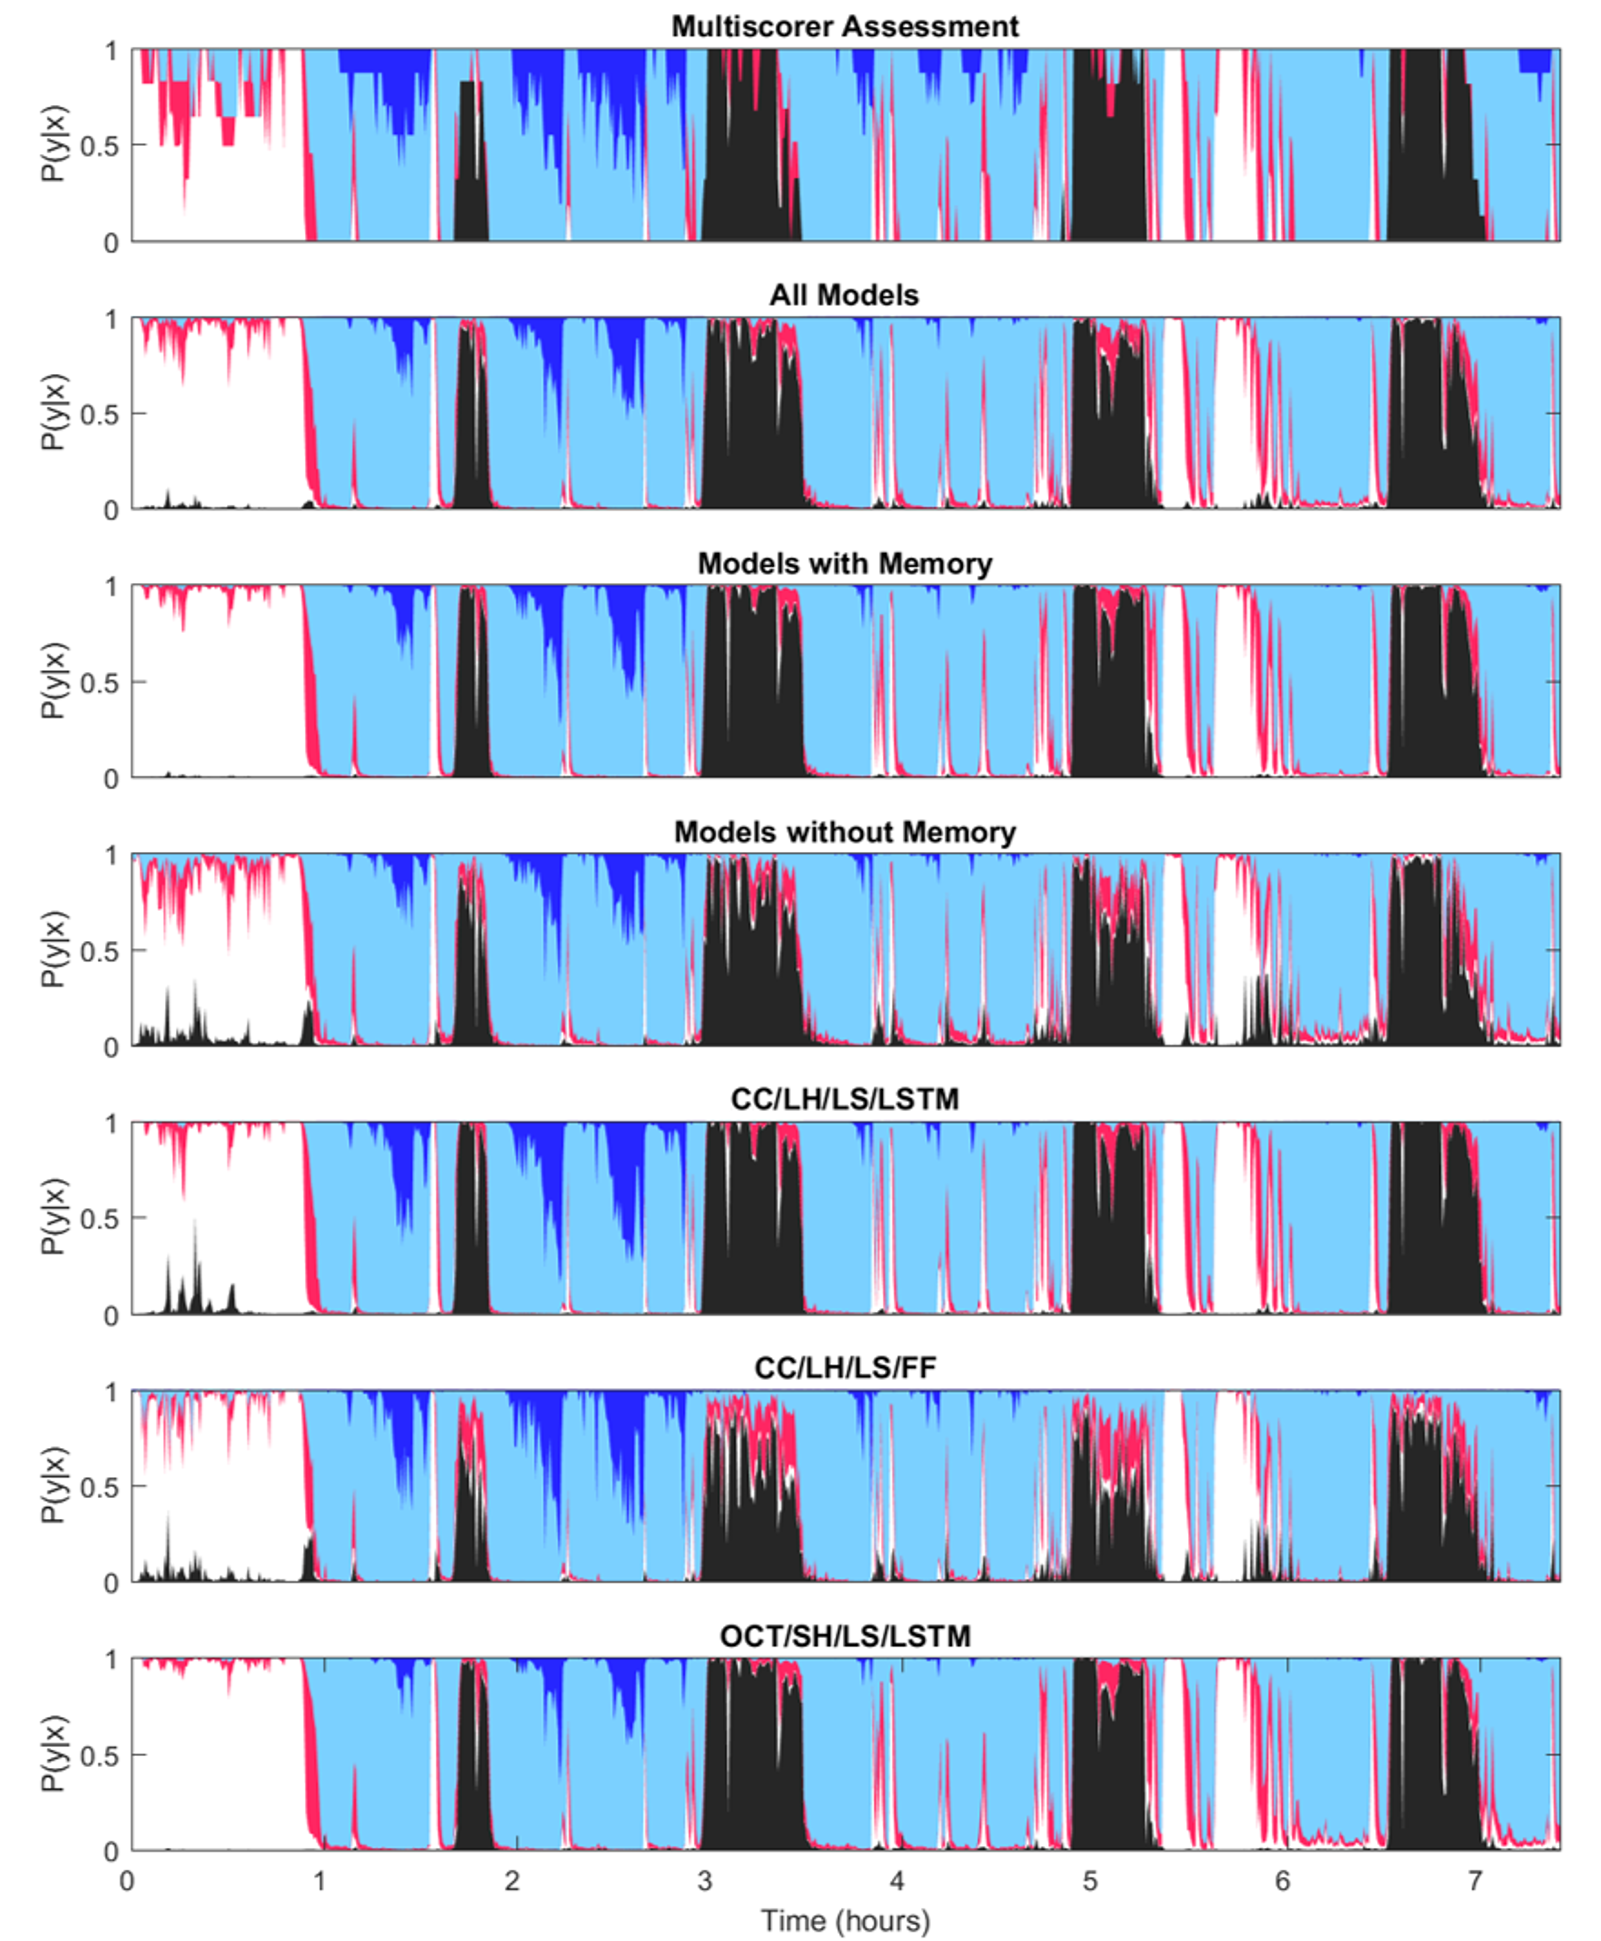
\includegraphics[width=\linewidth]{figures/paper-iii/Figure_2a}
    \caption[Hypnodensity example evaluated by different models]{The figure displays the hypnodensity graph. Displayed models are in order: multiple scorer assessment (1); ensembles: All models, those with memory (\ac{LSTM}) and those without memory (FF) (2–4); single models. OCT is octave encoding, Color codes: white, wake; red, \ac{N1}; light blue, \ac{N2}; dark blue, \ac{N3}; black, \ac{REM}.}
    \label{fig:sleep-stages:paper-iii:figure-02a}
\end{adjustwidth*}
\end{figure}

\begin{figure}
\begin{adjustwidth*}{}{-\marginparsep-\marginparwidth}
    % \centering
    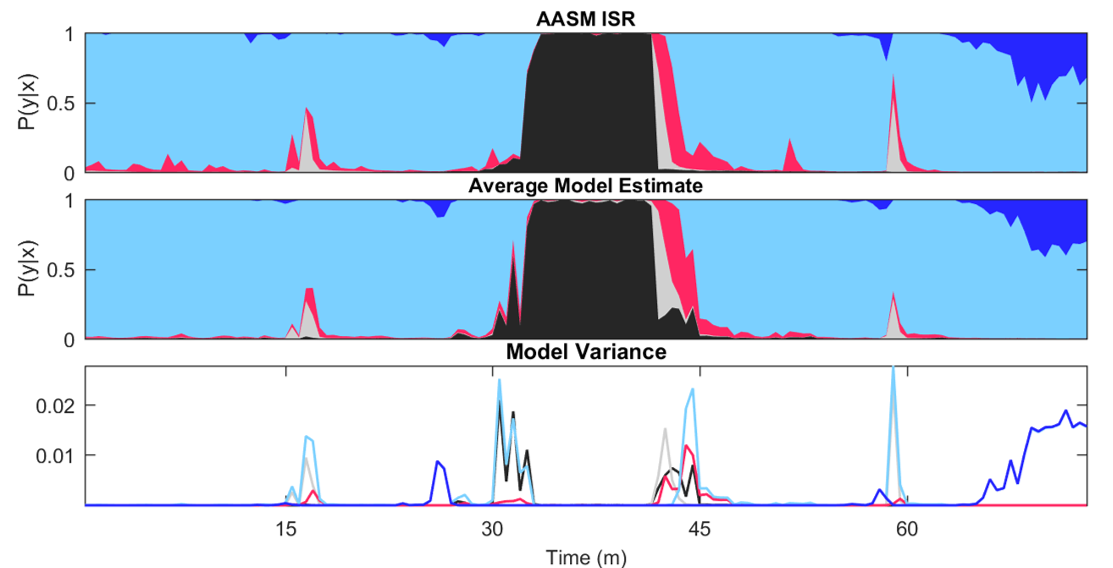
\includegraphics[width=\linewidth]{figures/paper-iii/Figure_2b}
    \caption[Evaluation of model on \acs{AASM} \acs{ISR}.]{The 150 epochs of a recording from the \ac{AASM} \ac{ISR} are analyzed by 16 models with randomly varying parameters, using the \ac{CC}/SH/LS/\ac{LSTM} model as a template. These data were also evaluated by \plusminus{5234}{14} different scorers. The distribution of these is shown on top, the average model predictions are shown in the middle, and the model variance is shown at the bottom.}
    \label{fig:sleep-stages:paper-iii:figure-02b}
\end{adjustwidth*}
\end{figure}
% \begin{figure}[!tb]
%     \myfloatalign   
%     \subfloat[]
%     {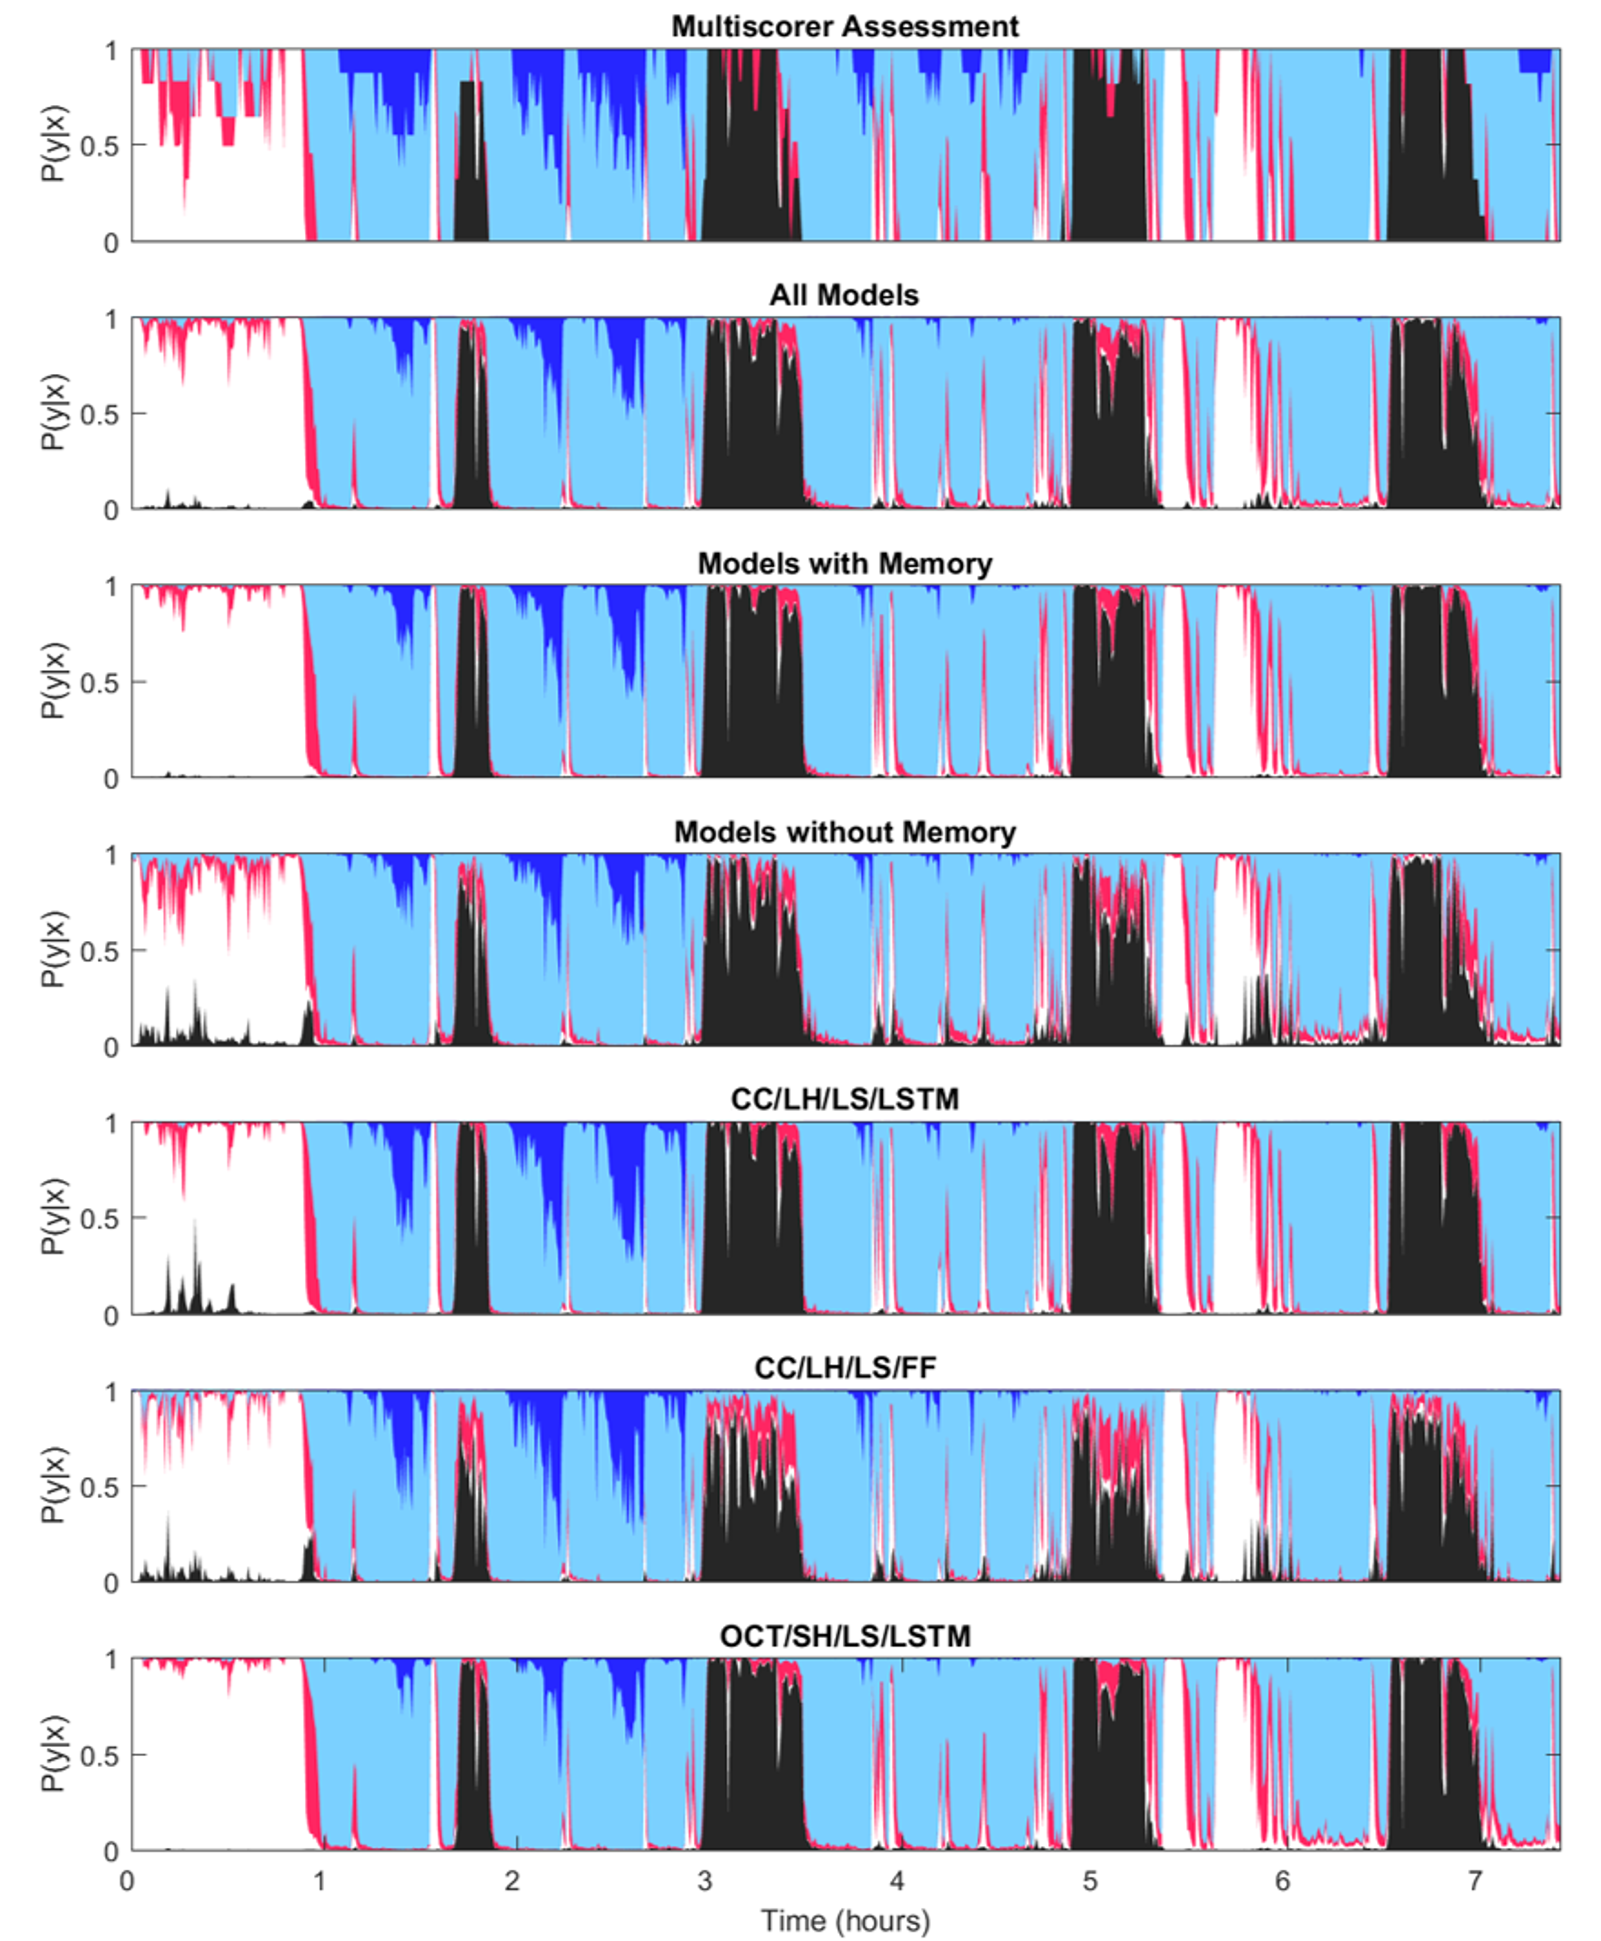
\includegraphics[width=\textwidth]{figures/paper-iii/Figure_2a}} \\
%     \subfloat[]
%     {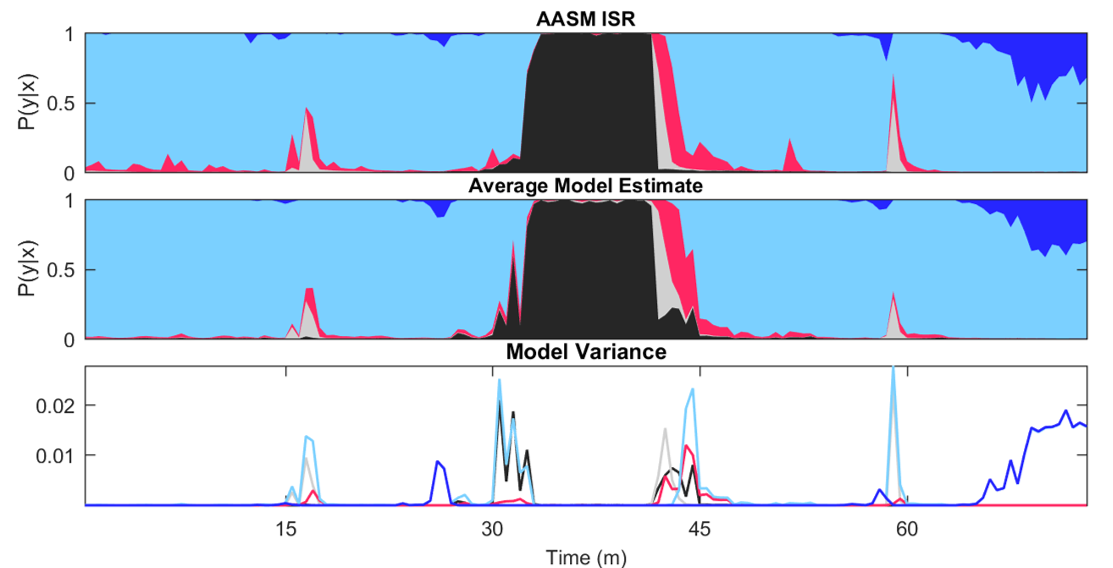
\includegraphics[width=\textwidth]{figures/paper-iii/Figure_2b}}
%     \caption[Hypnodensity example evaluated by multiple scorers and different predictive models]{Hypnodensity example evaluated by multiple scorers and different predictive models. (a)  b }
%     \label{fig:paperiii-figure02}
% \end{figure}

\subsubsection{Influences of sleep pathologies}
% As seen in Table 2, the different cohorts achieve different performances.
To see how much may be attributed to various pathologies, five different analyses of variance were made, with accuracy as the dependent variable, using cohort, age (grouped as age $<$ 30, 30 $\leq$ age $<$ 50, and age $\geq$ 50) and sex as covariates, investigating the effect of insomnia, OSA, restless leg syndrome (RLS), periodic leg movement index (PLMI) and \ac{NT1} on accuracy of our machine learning routine versus human scoring. 
This was performed in the cohort mentioned above with addition of the \ac{AHC}. 
The \textit{p}-values obtained from paired \textit{t}-testing for each condition were $0.75$ (insomnia), $7.53 \times 10^{-4}$ (OSA), $0.13$ (RLS), $0.22$ (PLMI) and $1.77 \times 10^{-15}$ (\ac{NT1}) respectively, indicating that only narcolepsy had a strong effect on scorer performance. 
Additionally, in the context of narcolepsy, cohort and age yielded \textit{p}-values between $3.69 \times 10^{-21}$ and $2.81 \times 10^{-82}$ and between $0.62$ and $6.73 \times 10^{-6}$, respectively. 
No significant effect of gender was ever noted. 
Cohort effects were expected and likely reflect local scorer performances and differences in \ac{PSG} hardware and filter setups at every site. 
Decreased performance with age likely reflects decreased \ac{EEG} amplitude, notably in \ac{N3}/slow wave sleep amplitude with age36.

\begin{figure}[tb]
\begin{adjustwidth*}{}{-\marginparwidth-\marginparsep}
    \myfloatalign   
    \subfloat[]
    {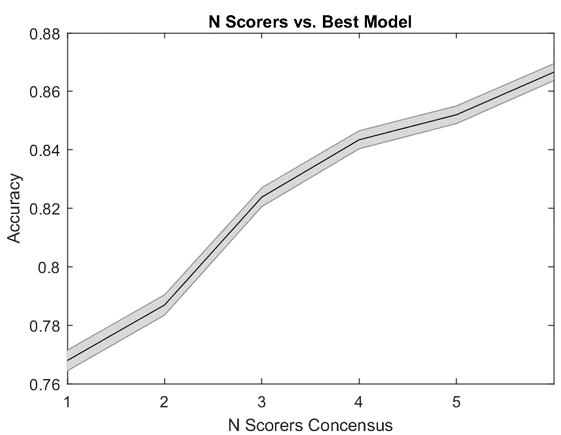
\includegraphics[width=0.48\linewidth]{figures/paper-iii/Figure_1a}}  ~
    \subfloat[]
    {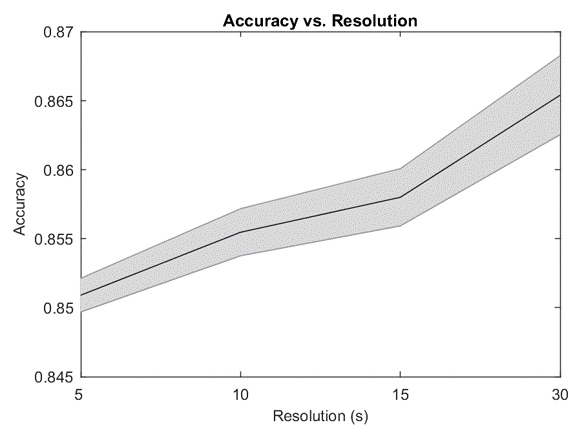
\includegraphics[width=0.5\linewidth]{figures/paper-iii/Figure_1b}}
    \caption[Accuracy per scorer and by time resolution]{Accuracy per scorer and by time resolution. (a) The effect on scoring accuracy as golden standard is improved. Every combination of $N$ scorers is evaluated in an unweighted manner and the mean is calculated. Accuracy is shown with mean (solid black line) and a 95\% confidence interval (gray area). (b) Predictive performance of best model at different resolutions. Performance is shown as mean accuracy (solid black line) with a 95\% confidence interval
(gray area).}
    \label{fig:sleep-stages:paper-iii:figure-01}
\end{adjustwidth*}
\end{figure}

\subsubsection{Resolution of sleep stage scoring}
Epochs are evaluated with a resolution of 30 s, a historical standard that is not founded in anything physiological, and limits the analytical possibilities of a hypnogram.
Consequently, it was examined to what extent the performance would change as a function of smaller resolution.
Only the models using a segment size of 5 s were considered.
Segments were averaged to achieve performances at 5, 10, 15 and 30 s resolutions, and the resulting performances in terms of accuracy are shown in~\cref{fig:sleep-stages:paper-iii:figure-01}b. 
Although the highest performance was found using a resolution of 30 s, performance dropped only slightly with decreasing window sizes.

\subsection{Discussion}
In recent years, machine learning has been used to solve similar or more complex problems, such as labeling images, understanding speech and translating language, and have seen advancement to the point where humans are now sometimes outperformed~\cite{Hinton2012b,He2015a,He2016}, while also showing promising results in various medical fields~\cite{Cheng2016,Gulshan2016,Bejnordi2017,Esteva2017,Lakhani2017,Ting2017}.
Automatic classification of sleep stages using automatic algorithms is not novel~\cite{Anderer2005, Fiorillo2019}, but only recently has this type of machine learning been applied and the effectiveness has only been demonstrated in a small numbers of sleep studies~\cite{Ronzhina2012,Lajnef2015,Olesen2016,Boostani2017,DaSilveira2017}. 
Because \acp{PSG} contain large amounts of manually annotated gold standard data, we hypothesized this method would be ideal to automatize sleep scoring.
We have shown that machine learning can be used to score sleep stages in \acp{PSG} with high accuracy in multiple physical locations in various recording environments, using different protocols and hardware/software configurations, and in subjects with and without various sleep disorders.

After testing various machine learning algorithms with and without memory and specific encodings, we found increased robustness using a consensus of multiple algorithms in our prediction.
The main reason for this is likely the sensitivity of each algorithm to particular aspects of each individual recording, resulting in increased or decreased predictability.
\Cref{fig:sleep-stages:paper-iii:figure-s01}b displays the correlations between different models.
Those incorporating an ensemble of different models generally have a higher overall correlation coefficient than single models, and since individual models achieve similar performances, it stands to reason that these would achieve the highest performance.

In addition to the stochastic nature of the training, one potential source for this variability was that recordings were conducted in different laboratories that were using different hardware and filters, and had \acp{PSG} scored by technicians of various skill levels.
Another contributor was the presence of sleep pathologies in the dataset that could influence machine learning.
However, of the pathologies tested, only narcolepsy had a very significant effect on the correspondence between manual and machine learning methods.
This was not surprising as the pathology is characterized by unusual sleep stage transitions, for example, transitions from wake to \ac{REM} sleep, which may make human or machine learning staging more difficult.
This result suggests that reporting inter-model variations in accuracy for each specific patient has value in flagging unusual sleep pathologies.

Unlike previous attempts using automatic detector validations, we were able to include 70 subjects scored by 6 technicians in different laboratories from the \ac{IS-RC} to independently validate our best automatic scoring consensus algorithm~\cite{Kuna2013}.
This allowed us to estimate the performance at 87\% in comparison to the performance of a consensus score for every epoch among six expert technicians, see~\cref{tab:sleep-stages:paper-iii:table-01}.
Including more scorers produces a better gold standard, and as~\cref{fig:sleep-stages:paper-iii:figure-01}a indicates, the model accuracy also increases with more scorers.
Naturally, extrapolating from this should be done with caution; however, it is reasonable to assume that the accuracy would continue to increase with increased scorers.
In comparison, performance of any individual scorer ranges from 74 to 85\% when compared to the same six-scorer gold standard, keeping in mind this performance is artificially inflated since the same scorers evaluated are included in the gold standard\graffito{The unbiased performance of any scorer versus consensus of remaining 5 scorers range from \SIrange{69}{80}{\percent}.}. 
The best model achieves 87\% accuracy using 5 scorers and achieves statistically significantly higher performance values than all scorers, as shown in~\cref{fig:sleep-stages:paper-iii:figure-01}a and \cref{tab:sleep-stages:paper-iii:table-01}.

As with human scorers, the biggest discrepancies in machine learning determination of sleep stages occurred between wake versus \ac{N1}, \ac{N1} versus \ac{N2} and \ac{N2} versus \ac{N3}.
This is logical as these particular sleep stage transitions are part of a continuum, artificially defined and subjective.
To give an example: an epoch comprised of 18\% slow wave activity is considered \ac{N2} while an epoch comprised of 20\% slow wave activity qualifies as \ac{N3} according to \ac{AASM} guidelines~\cite{Berry2020}.
Overall, data indicate that our machine learning algorithm performs better than individual scorers, as typically used in clinical practice, or similar to the best of 5 scorers in comparison to a combination of 5 experts scoring each epoch by consensus.
It is also able to score at higher resolution, i.e., 5 s, making it unnecessary to score sleep stages by 30 s epochs, an outdated rule dating from the time sleep was scored on paper.

In conclusion, models which classify sleep by assigning a membership function to each of five different stages of sleep for each analyzed segment were produced, and factors contributing to the performance were analyzed. 
The models were evaluated on different cohorts, one of which contained 70 subjects scored by 6 different sleep scoring technicians, allowing for inter-scorer reliability assessments.
The most successful model, consisting of an ensemble of different models, achieved an accuracy of 87\% on this dataset, and was statistically better performing than any individual scorer.
It was also able to score sleep stages with high accuracy at lower time resolution (5 s), rendering the need for scoring per 30 s epoch obsolete.
When predictions were weighted by the scorer agreement, performance rose to 95\%, indicating a high consensus between the model and human scorers in areas of high scorer agreement.
A final implementation was made using an ensemble with small variations of the best single model.
This allowed for better predictions, while also providing a measure of uncertainty in an estimate.
